\chapter[干渉]
{干渉}


\chaptermark{干渉}

\section{強め合う干渉と弱め合う干渉}
まずは重ね合わせを見てみましょう。単一周波数の波を見てみましょう.
それがまずは時間通りに空中を通る波を見てみましょう:
c
これが数式になるんですけれども$E$はこの瞬間の波の振幅になります。
\begin{itemize}
    \item $E_0$が波のAmplitude 振幅のなんですが、それが最大の振幅です。
    \item あとはこれが$sin$の波になりますから$sin(\omega t  - (k x + \phi))$なんですが こういう定義にしましょう
    \item $\omega$が角周波数ですね。そうすると$\omega = \frac{2\pi}{T}$なんです。
    \item $k$はwave numberになるんですけれどもそれ(波)の数なんで$k=\frac{2\pi}{\lambda}$なんです。
    \item $\phi$は初期位相、最初の位相になります。
    \item $\lambda$が波長、それが波の長さなんです。
    \item あと大文字のTがperiodになりますね。そのperiodが周期です。

\end{itemize}
%E_0がそれが言ってた通りで
%振幅のの最大の大きさなんですが

そうするとじゃあこれがちょっと見てみましょう:

こんな感じになるんですが:
% k=1, k=0
\begin{figure}[H]
   \centering
    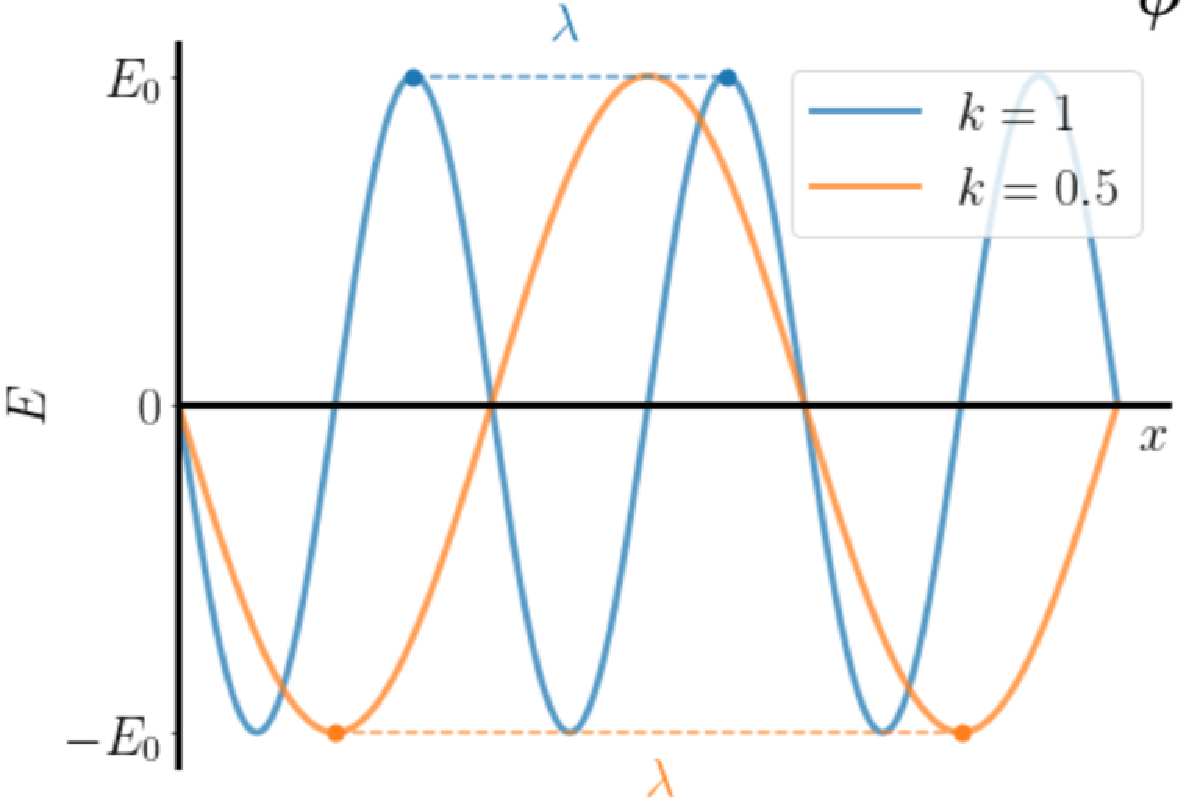
\includegraphics[width=0.8\textwidth]{lesson6/k.pdf}
    \label{fig: 1}
    \begin{center}
        \caption{$k=1, k=0.5$の波}
    \end{center}
\end{figure}

各所には青い波とオレンジ色の波なんですがえっと、2つともあの最初の瞬間でまぁこの波は連続になっているんですけれどもこれが永遠の昔から永遠の未来まで波が連続している状態なんです。$t=0$の瞬間の波の状態ちょっと見てみましょう。そうすると、この2つの波が一つはwave number が $k = 1$ で
もう一つは wave number $k = 0.5$。つまり半分になります。
そうすると、二つの隣あう波の最も高くなっている点の間の距離が$\lambda$なんですがその$\lambda$は波長、波の長さ。それが最大のところから最小に落ちるんですけれどもその戻ってくるところまで、それが波長になります。

そうすると、それが $k = 1$ の場合なんですが
$k = 0.5$ の場合だったらそれはもどって来るレイトがその半分になる。まあ僕は最初には、てっぺんのところで説明してたんですけれども\textbf{Figure 6.2}によると、 0に戻る例で見てみましょう。で、青いの波が0に始まって下にいて1回戻ってきてもう一回戻ってくるとそれがオレンジの波がが一回だけ戻ってきているでしょ。つまりその進むペース、位相が変わるペースは半分になっている。

そうすると、あの位相が変わる例を見てみましょう:
% phi = 0, phi = pi/2
\begin{figure}[H]
   \centering
    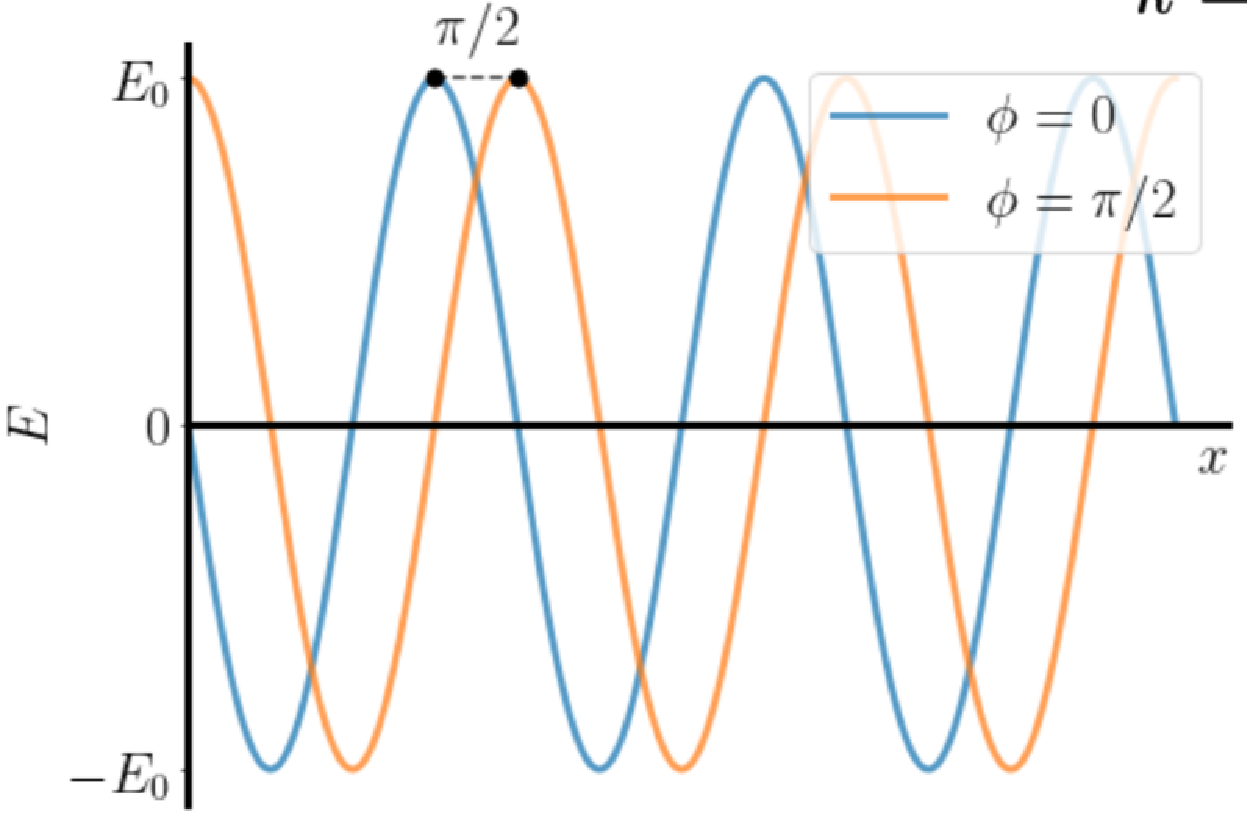
\includegraphics[width=0.8\textwidth]{lesson6/phi.pdf}
    \label{fig: 1}
    \begin{center}
        \caption{$\phi = 0, \phi = \pi / 2$ の波}
    \end{center}
\end{figure}
そのそれが初期位相なんですが最初の、どこから始まったかということなんです。つまりこの場合には、$\phi = 0$と$\phi = \frac{\pi}{2}$の波が
2つとも形は一緒なんですが、始まったところは別で一つはオレンジが上のところで始まって青のやつは下の0のところで始まったから最初にでは2つとも落ちているんですけれども青い波が、それが逆転して上がっていくところにはそれがもっと早くそのターンにはなりますよね。そうすると、時間を見てみましょう。

これが時間に依存なんですがこれが一つの波だけ見てみましょう:
% gif two waves [insert pic]
\begin{figure}[H]
   \centering
    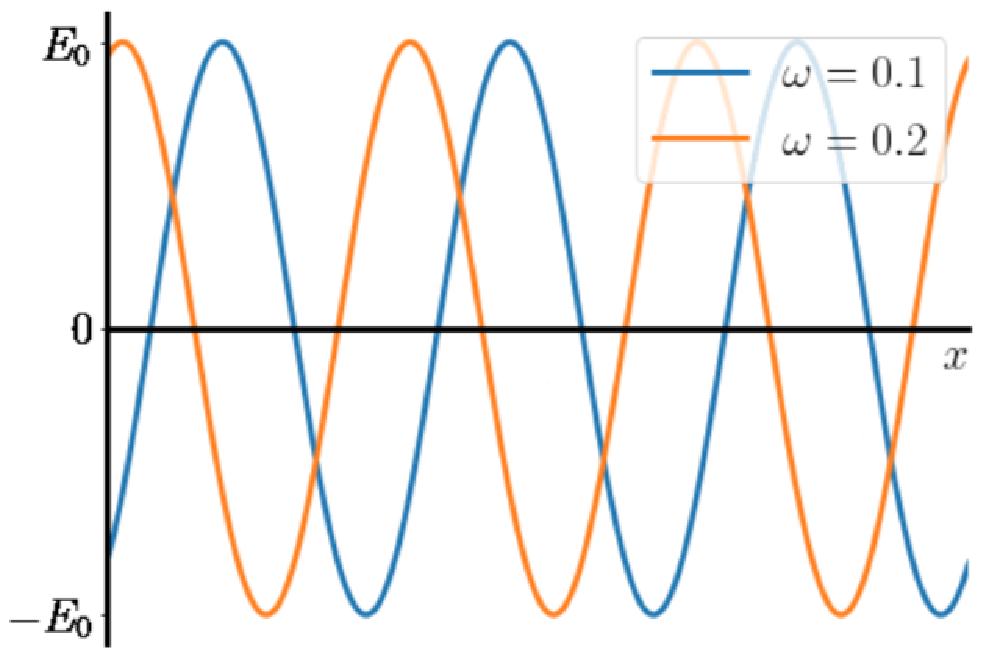
\includegraphics[width=0.8\textwidth]{lesson6/w.pdf}
    \label{fig: 1}
    \begin{center}
        \caption{$\omega = 0.1, \omega = 0.2$ の波}
    \end{center}
\end{figure}

これが$k = 1$の場合で数学的には簡単になるんですが、まあもっと汎用的にも言えると思うんで、えっと$\phi=0$の場合には波はこういうふうに進みますね。これが二つの例の波が入ってるんですが一つの$\omega$、周波数なんですがその周波数が0.1ともう一つは0.2になります。二つを見ると、まあこういう場合に見ると、 
あの速い方は 速く進んでいる気がするでしょ。
\subsection{二つの波の重ね合わせ}
そうすると干渉に向かっているので 2つの波を例に見てみましょう:
\begin{equation}
\begin{array}{ll}
E_{1}=E_{01} \sin \left(\omega t+\alpha_{1}\right), & \alpha_{1}=-\left(k x+\phi_{1}\right) \\
E_{2}=E_{02} \sin \left(\omega t+\alpha_{2}\right), & \alpha_{2}=-\left(k x+\phi_{2}\right)
\end{array}
\end{equation}

じゃあえっと、まずはこの例は二つともこの瞬間的な振幅が$E_1$と$E_2$といって、これは$E_{01}$が最大の振幅で$E_{02}$は2つ目のwaveの最大の振幅なんですが、あともうちょっと簡単な表現にすると$\omega t + \alpha$、それを$\alpha_{1}$と$\alpha_{2}$にするんですが、(この場合は、) 二つとも同じ周波数の$\omega$になります。

で、これの結果の波を考えるとまぁ各地のいろいろところはすべてのところエリアには波1と波2の足し算になりますから、 
それがあとこれが線形の関数ですが足し合わせになりますが、
それが $E = E_1 + E_2$ になります。

そうするとこれがまあ最初にはこの二つの表現があるんですけれどもそれを、もうちょっとあの代数をちょっとやってみてその代数によって
こういう数式を作りたい:
\begin{equation}
E = E_0 sin(\omega t - \alpha)
\end{equation}
の場合にはこれが作れるかどうかちょっと見てみましょ。さてそれがそうすると、
$E_0$と$\alpha$を計算しなければならないんですよね。この上の表現からそうするとこの$E$の場合はこういう表現になります:
\begin{equation}
\begin{aligned}
E &=E_{01}\left(\sin \omega t \cos \alpha_{1}+\cos \omega t \sin \alpha_{1}\right) \\
&+E_{02}\left(\sin \omega t \cos \alpha_{2}+\cos \omega t \sin \alpha_{2}\right)
\end{aligned}
\end{equation}
これが上の行は波1のcontributionと二行目が波2のcontributionになるんですけども、これが基本的に$sin\omega t cos\alpha_{1}  + cos\omega t sin \alpha_{1} $ 
これがあの三角関数の公式を使ってこれが計算できるようになりますこれが、細かくは説明しないんですけれどもしかして良い課題になるかもしれないんですね。
その上の表現からからこの後の表現までの代数をやってみるのも、良いと思います。
さてこれが、時間依存の表現にちょっと分けてみましょう:
\begin{equation}
\begin{aligned}
E &=\left(E_{01} \cos \alpha_{1}+E_{02} \cos \alpha_{2}\right) \sin \omega t \\
&+\left(E_{01} \sin \alpha_{1}+E_{02} \sin \alpha_{2}\right) \cos \omega t
\end{aligned}
\end{equation}

\iffalse
これが sin$\omega$t は左の青いところにあるので
cos$\omega$t は右側のオレンジ色に囲まれている
\fi
さて そうするとこの場合には:
\begin{equation}
\begin{aligned}
&E_{0} \cos \alpha=E_{01} \cos \alpha_{1}+E_{02} \cos \alpha_{2} \\
&E_{0} \sin \alpha=E_{01} \sin \alpha_{1}+E_{02} \sin \alpha_{2}
\end{aligned}
\end{equation}
\iffalse
E_0cos\alpha はこの表現になるんですが 
E_01cos\alpha1 +  E_02 cos\alpha2

0:09:08.123,0:09:19.190
と、E_0sin\alpha =  E_01sin\alpha1 + E_02sin\alpha2
なんですが
\fi
そうすると、まあこれが$E_0$を計算したいので次のステップにはどうするべきでしょう?まあ三角関数の公式を使うと、$cos^{2} + sin^{2} = 1$にしますから、
2つともとも二乗にると、
こういう表現ができるようにはなります:
\begin{equation}
\begin{aligned}
&E_{0}^{2}=E_{01}^{2}+E_{02}^{2}+2 E_{01} E_{02} \cos \left(\alpha_{2}-\alpha_{1}\right) \\
&\tan \alpha=\frac{E_{01} \sin \alpha_{1}+E_{02} \sin \alpha_{2}}{E_{01} \cos \alpha_{1}+E_{02} \cos \alpha_{2}}
\end{aligned}
\end{equation}
\iffalse
0:09:50.000,0:09:57.607
E_0^2 = E_01^2 +E_02^2 + なんとかなんとかにすると

0:09:57.607,0:10:01.889
下の行には、
tan\alphaになります。
\fi
こういうふうにすると、 $E_0$と$tan\alpha$を計算できるようになります。
さて、重ね合わせを見てみましょう:
\begin{equation}
E = E_0 sin(\omega t + \alpha)
\end{equation}
これが、重ね合わせは、各周波数がそれのcomponentの波と一緒になりますけれどもその$\omega$は変わらないんですよね、ですが振幅と位相が変わります:
\begin{equation}
E_{0}^{2}=E_{01}^{2}+E_{02}^{2}+2 E_{01} E_{02} \cos \left(\alpha_{2}-\alpha_{1}\right)
\end{equation}
そうすると、これがさっきのスライドで計算した$E_0$のことなんですが最初の$E_{01}^{2}$、$E_{02}^{2}$これが変われないんですけれども、
この後 $2 E_{01} E_{02} \cos (\alpha_{2}-\alpha_{1})$、これが干渉のtermになりますね、干渉の表現になります。するとこれは$\alpha_1$ と $\alpha_2$ の差に依存するでしょ。
これが $\delta$(デルタ) という表現を使ったら
\begin{equation}
    \delta = 0, \pm2\pi, \pm4\pi, \pm6\pi, \pm8\pi, \pm10\pi
\end{equation}
のように連続するとこれが、\textbf{constructive interferenceこれが、強め合う干渉になります。}

そうすると逆の方には
\begin{equation}
    \delta = \pm1\pi, \pm3\pi, \pm5\pi
\end{equation}
 になると、\textbf{これが弱め合う干渉になります
destructive interference になります。}

じゃあ例を見てみましょう:
\begin{equation}
\begin{aligned}
&E_{1}=\sin (0.1 t-x) \\
&E_{2}=\sin (0.1 t-0.8 x) \\
&E=E_{1}+E_{2}
\end{aligned}
\end{equation}

これは、例えば波1が、まあ二つとも $\omega = 0.1$にしているんですけれども
波の数が、一つは1になっているともう一つは0.8になっているとこういうふうになります。重ね合わせ。
% superposition two waves
\begin{figure}[H]
   \centering
    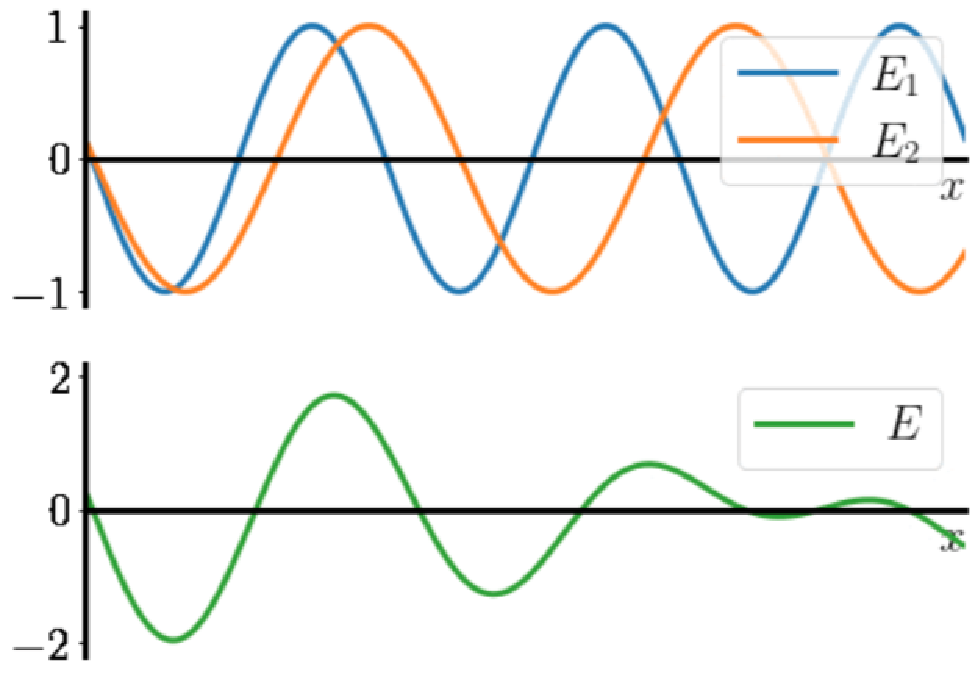
\includegraphics[width=0.8\textwidth]{lesson6/wave_superposition.pdf}
    \label{fig: 1}
    \begin{center}
        \caption{重ね合わせ状態の波}
    \end{center}
\end{figure}

上の図は、 これが2つの波を各波としてプロットしているんですけれども
下の方はそれが足し算してその足し算はこういうアウトプットの関数になります。
そうすると、あるところは強くなってますし、あるところ弱くなっているでしょう。これは、強め合うと弱め合うの干渉になります。概念は見たことあると思いますけれどももうちょっと定量的に見てみましょう。



\section{位相速度と群速度}
% \subsection{位相速度}
波の普通の速度なんですけど、それが変わらない位相には、それがどれくらい速く進んでいるのかという定義なんですけど、この場合だったら:
\begin{equation}
E=E_{0} \sin (\omega t-k x-\phi)
\end{equation}


$\theta=\omega t-k x-\phi$がPhaseになるんですが、これが位相になりますよね。sinの引数になっているので$\omega t - k x - \phi$ですよね。

そうすると 、$v$、これが\textbf{ wave の velocity、 波の速度}なんですが、それが$\frac{\lambda}{T}$になります。$\lambda$ は波長ですよね。 大文字のTはperiod になりますよね。一つの波が0からいって、$2\pi$にいって戻ってくる時間ですね。

で、えっと、$\lambda$の場合には$\lambda = \frac{2\pi}{k}$ と
Tだったら、$T = \frac{2\pi}{\omega}$すると、その速度が、$v =\frac{\omega}{k}$ ですね。
これがちょっとみてみましょう:
\begin{equation}
E=\sin (0.1 t-x)
\end{equation}
にするとグラフは下の感じなんですが、こういうphase velocityこれが位相速度なんです:
% graph, black dot
\begin{figure}[H]
   \centering
    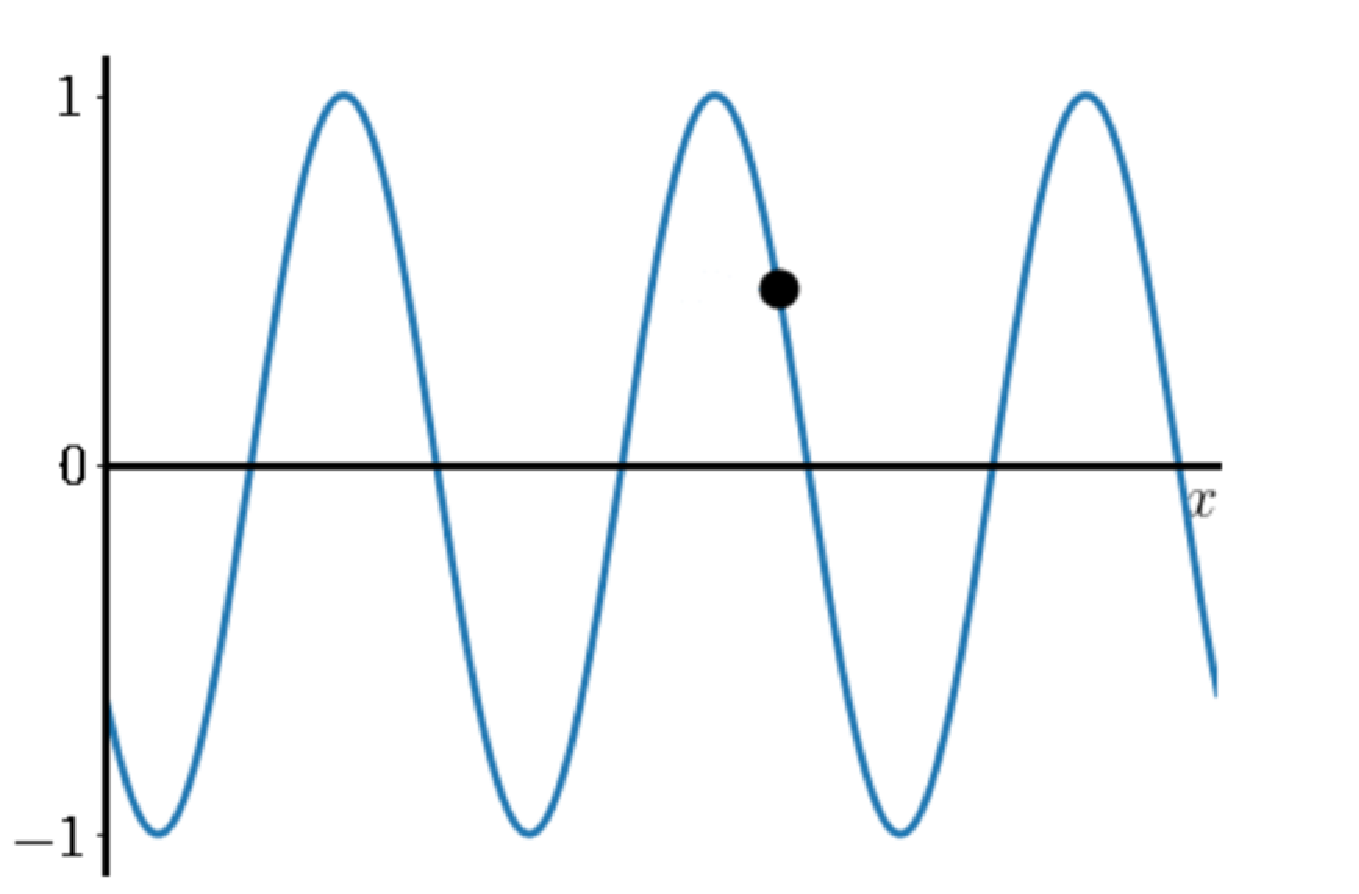
\includegraphics[width=0.8\textwidth]{lesson6/black_dot.pdf}
    \label{fig: 1}
    \begin{center}
        \caption{一つの波の位相速度}
    \end{center}
\end{figure}
黒い丸がありますよね。この赤い丸がこのペースで進んでいると、これがどのくらいの速さで進んでいるのか。それが、位相速度。同じところでどのくらい速く進んでいるのか。同じ高さ、同じ振幅なんですが、そうすると 、じゃあ重ね合わせではどうなるでしょうかね:
% Aug 15 11:30 ここまで
一つの波だったら簡単な例になるんですけれども、二つ合わせると前のステップの終わりのところで、ちょっと見たんですが波の高さが変わってしまうでしょう。強め合うと、弱め合うの干渉になりますから定義が変わってしまいますね:
\begin{equation}
\begin{aligned}
&E_{1}=E_{0} \sin \left(\omega_{1} t-k_{1} x\right) \\
&E_{2}=E_{0} \sin \left(\omega_{2} t-k_{2} x\right)
\end{aligned}
\end{equation}
さっきのステップの例をちょっと改善して$E_1$と$E_2$、これが波1と波2なんですが(この場合、)二つの波の振幅は同じなので$E_0$になります。
そうすると 、その重ね合わせはこういう複雑な表現になります:
\begin{equation}
\begin{aligned}
E &=E_{1}+E_{2} \\
&=E_{0}\left[\sin \left(\omega_{1} t-k_{1} x\right)+\sin \left(\omega_{2} t-k_{2} x\right)\right] \\
&=2 E_{0} \sin \left[\frac{\omega_{1}+\omega_{2}}{2} t-\frac{k_{1}+k_{2}}{2} x\right] \\
& \times \cos \left[\frac{\omega_{1}-\omega_{2}}{2} t-\frac{k_{1}-k_{2}}{2} x\right]
\end{aligned}
\end{equation}
これも、各表現については説明しないんですが、信じていただければと思います。もうちょっとみてみると、2つのtermに分けられますが、$sin$のtermと$cos$のtermに分けられますね。これが、まあ代数と三角関数なんですけれども計算はあっという間には見当たらないかもしれないですけど信じていただければと思います。
\begin{equation}
E=2 E_{0} \sin \left[\frac{\omega_{1}+\omega_{2}}{2} t-\frac{k_{1}+k_{2}}{2} x\right] \times \cos \left[\frac{\omega_{1}-\omega_{2}}{2} t-\frac{k_{1}-k_{2}}{2} x\right]
\end{equation}
そうすると 、\textbf{式6.17}を、2つNI分けて、一つ目の項は、$\omega_1 + \omega_2$になってますよね。と、$k_1 + k_2$ になってますよね。
このところには、\textbf{振動するところは、速くなります}。それが左側なんです。

\textbf{右側は、これがゆっくりに行きます}。これが、$\omega_1 - \omega_2$と $k_1 - k_2$。そうすると 、上の項の差に依存するでしょ。左が足し算に依存するけど、右が引き算に依存する。

そうすると 、じゃあこの場合にはさっきの位相速度はどういう風に定義しましょうか?これが、$v_p$といいますが、\textbf{phase velocity}。これが、
\begin{equation}
v_p = \frac{\omega_{1}+\omega_{2}}{k_{1}+k_{2}}
\end{equation}
で、\textbf{Group velocity} これが $v_g$ 。
このGroup velocityは群速度で:
\begin{equation}
v_g = \frac{\omega_{1}-\omega_{2}}{k_{1}-k_{2}}
\end{equation}
それが、fast oscillations  と slow oscillationsの関連になるでしょう。
この場合は、$v_p = v_g$ ではないですが、波が一つだけになってれば、単一の波だったら
$v_p$と$v_g$は一緒なんですが、これが、重ね合わせの場合には、絶対そうだとは言えない。

じゃあ例として具体的にみてみましょう:
\begin{equation}
\begin{aligned}
&E_{1}=\sin (0.1 t-2.0 x) \\
&E_{2}=\sin (0.2 t-2.1 x)
\end{aligned}
\end{equation}
\iffalse
二つの波で、一つは \omega = 0.1
でもう一つは \omega = 0.2 

0:05:40.609,0:05:48.658
で波の数が2.0と2.1
\fi
\textbf{式6.20}の式を足し算すると、こういう表現になるでしょう:
% t = 0 graph
\begin{figure}[H]
   \centering
    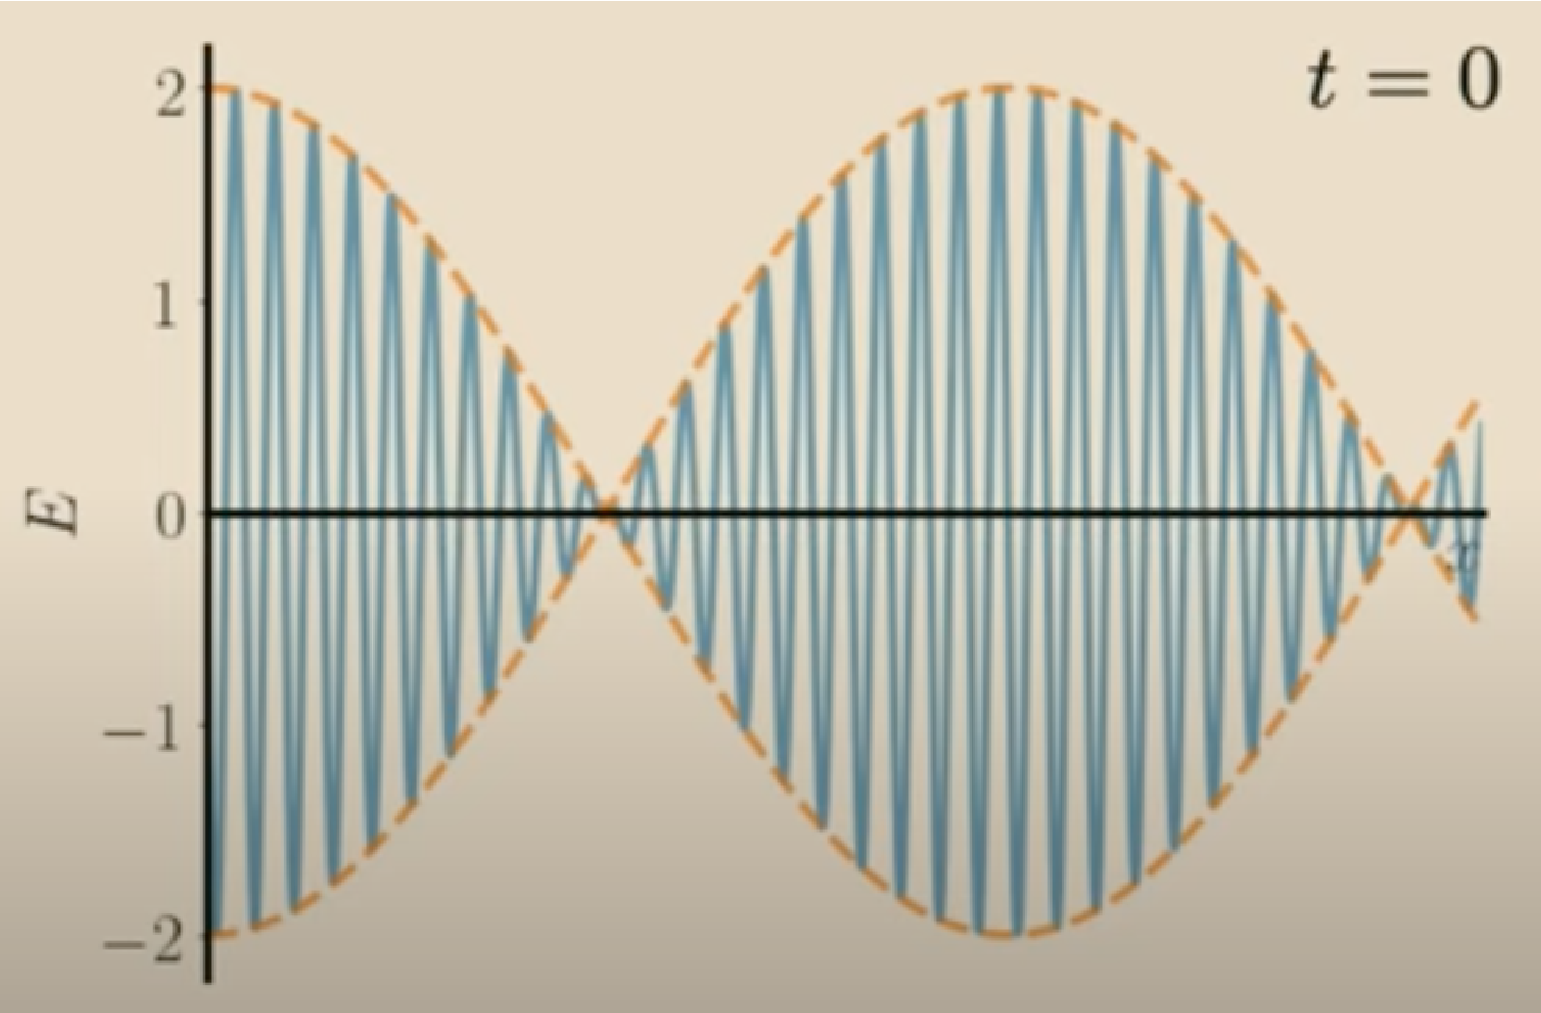
\includegraphics[width=0.8\textwidth]{lesson6/t=0.pdf}
    \label{fig: 1}
    \begin{center}
        \caption{一つの波の位相速度}
    \end{center}
\end{figure}

これが、まああの見えるところなんですけれども、足し算が、この速くなっている青い線なんですが、もう一つが、ゆっくり上がっていてゆっくり下がっていっているでしょう。こういうふうに、下から上がってきて、下に行くとそれが遅い周波数で、真ん中にある青いところ(波)が、もっと速いところです。これが$t = 0$の瞬間になります。
\iffalse
そうすると、動かすと、これは時間が経過しているんですが、こういう風に進むことになります。
じゃあ、こうすると、干渉が見やすいと思いますが、
0:06:53.308,0:06:54.610
えっと、
\fi
もうちょっと見てみるとこの場合だったら、\textbf{式1.18/1.19}の数式に入れるとphase velocity と group velocity は計算できます:
\begin{equation}
\begin{gathered}
v_{p}=\frac{\omega_{1}+\omega_{2}}{k_{1}+k_{2}}=\frac{0.3}{4.1} \approx 0.07 \\
v_{g}=\frac{\omega_{1}-\omega_{2}}{k_{1}-k_{2}}=1 & \begin{array}{l}
\end{array} \\
v_{g}>v_{p} \quad v_{g} \approx 14 v_{p}
\end{gathered}
\end{equation}
\iffalse
0:07:07.596,0:07:16.478
phase velocity 位相速度が 0.07 くらいになりますし

0:07:16.478,0:07:22.079
group velocity はこの場合には 1 になります。

0:07:22.079,0:07:32.344
\fi
この場合にはgroup velocity が phase velocityよりも速いんですが(群速度は位相速度より速い)というのは、大体14倍くらい速くなります。もう一回見てみましょう:
% red square, black dot
\begin{figure}[H]
   \centering
    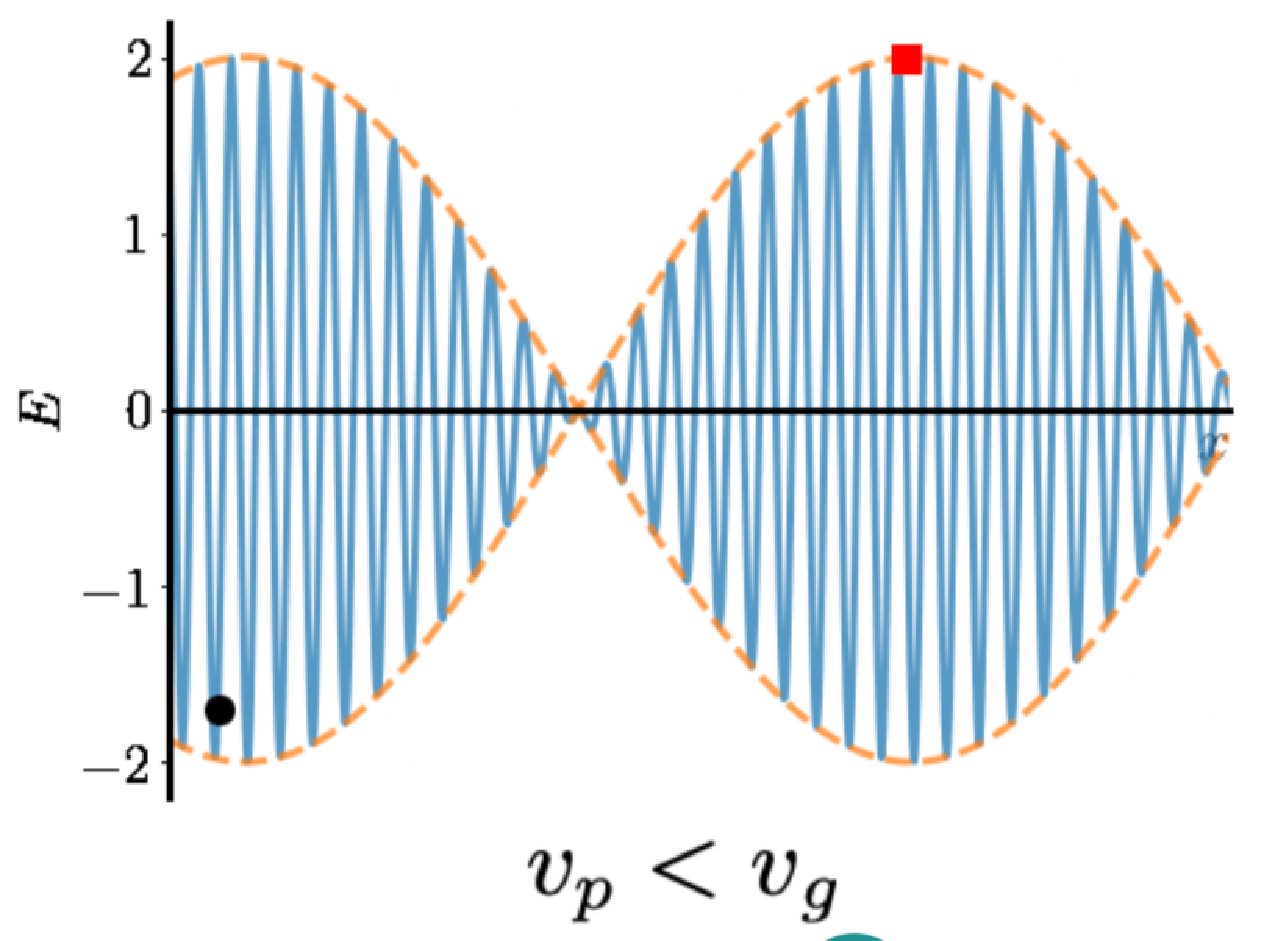
\includegraphics[width=0.8\textwidth]{lesson6/vp_less_vg.pdf}
    \label{fig: 1}
    \begin{center}
        \caption{$v_p < v_g$ 重ね合わせ状態}
    \end{center}
\end{figure}

そうすると、えっと群の速度は赤い四角です。位相の速度はもっとゆっくりと動いているので位相の速度はこの黒い丸のところなのです。という理由は、完全に独立ではないですが、違いがあるというのは自然なことです。
そうすると、この真ん中の振幅がこの重ね合わせの振幅はこの位大きくなっていますがそれが青い波なんですがこのオレンジ色の波が、波の\textbf{焙烙線、
wave envelope} と言いますね。この場合には、さっき言ってた通りでphase velocity は group velocityより遅い場合。

それだけとは限らないんですけれども、別の例を見てみましょう:
\begin{equation}
\begin{aligned}
&E_{1}=\sin (0.1 t-0.1 x) \\
&E_{2}=\sin (0.2 t-0.2 x)
\end{aligned}
\end{equation}
\iffalse
0:09:01.923,0:09:10.318
\omega が 0.1と 0.2 の波なんですが、

0:09:10.318,0:09:15.437
wave number も 0.1 と 0.2 にすると、
\fi
各波が進んでいるペースは一緒になるますが、重ね合わせになると、この二つの波が、複数の波があるように見えますが、この場合だったら、形は変わってないですよね:
% vp = vg
\begin{figure}[H]
   \centering
    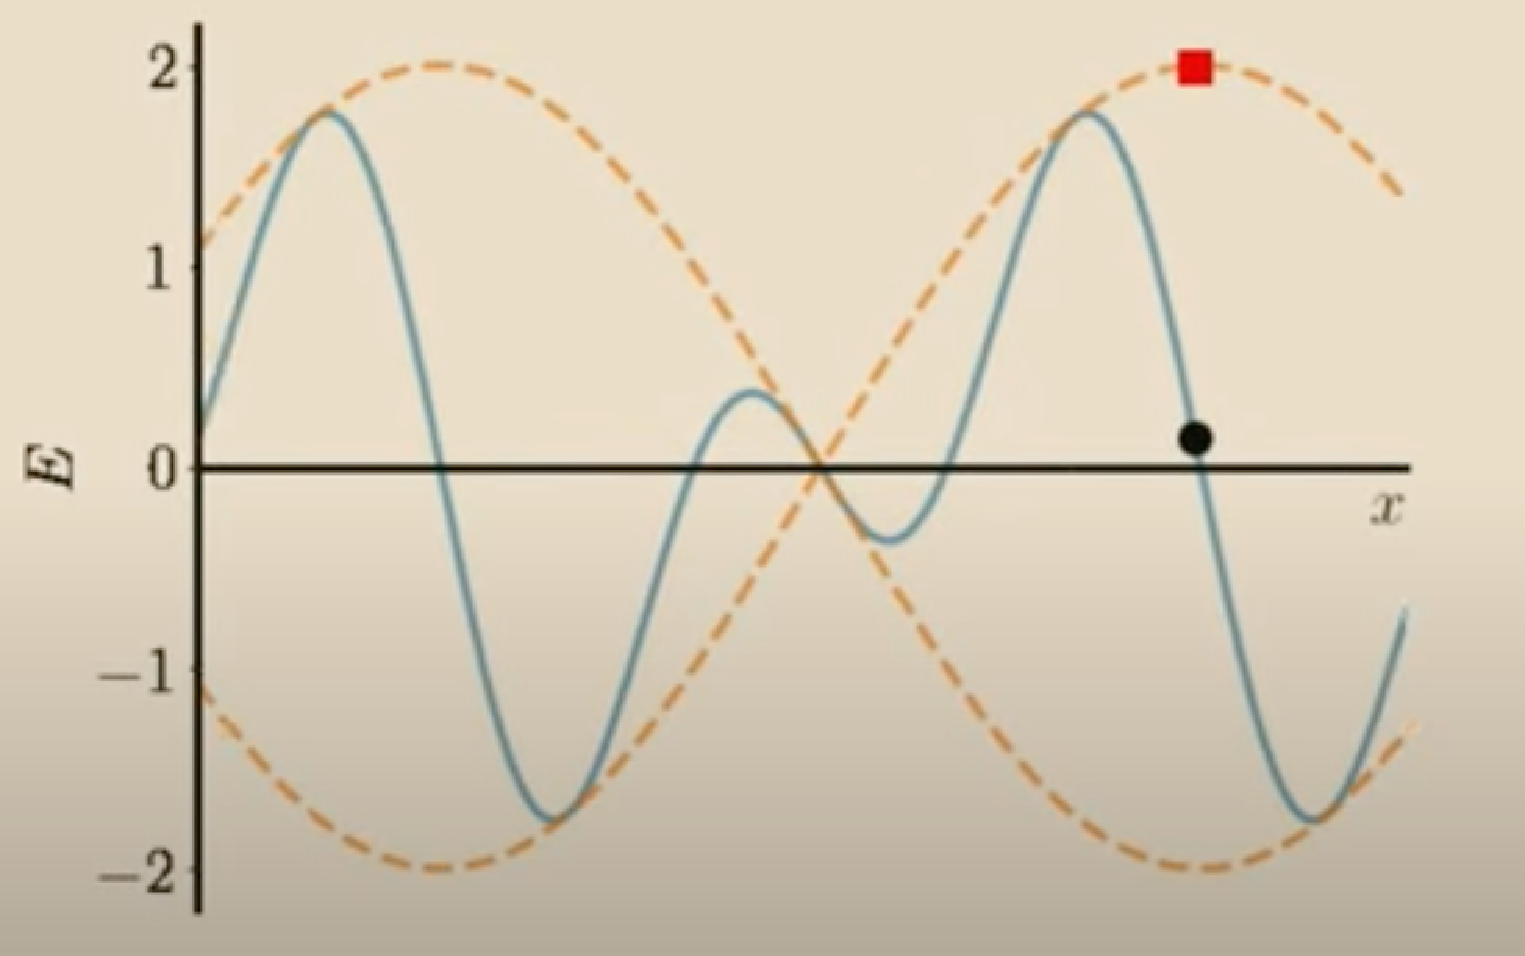
\includegraphics[width=0.8\textwidth]{lesson6/vp_equal_vg.pdf}
    \label{fig: 1}
    \begin{center}
        \caption{$v_p = v_g$ 重ね合わせ状態}
    \end{center}
\end{figure}
この場合には、位相速度と、群速度は一緒になります。

さて、群速度が速い場合もありますし、一緒の場合もありますし、もう一つの例だったら、それより遅い場合もあるかもしれないでしょ:
\begin{equation}
\begin{aligned}
&E_{1}=\sin (0.1 t-2.0 x) \\
&E_{2}=\sin (0.2 t-1.5 x)
\end{aligned}
\end{equation}
% vg < vp
\begin{figure}[H]
   \centering
    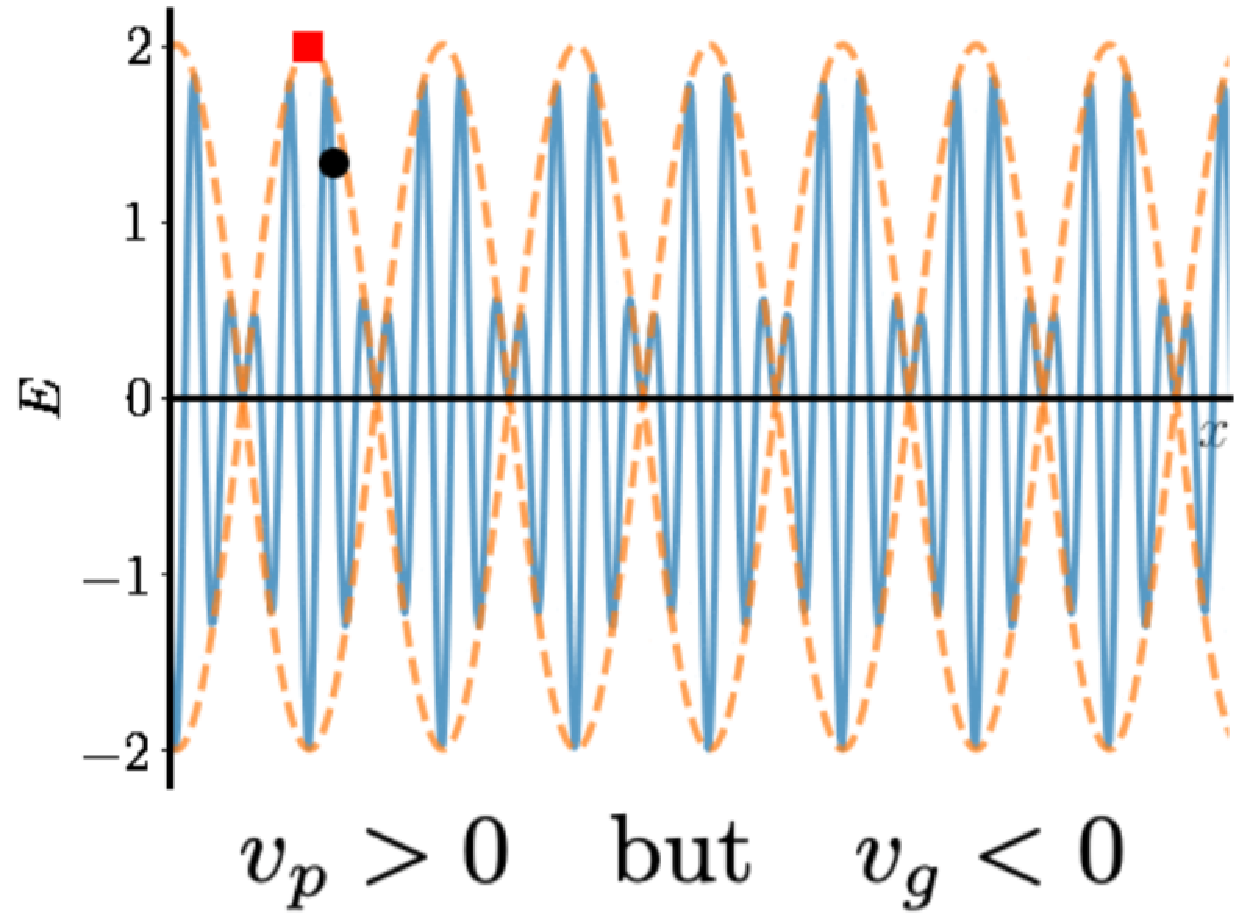
\includegraphics[width=0.8\textwidth]{lesson6/vp_greater_vg.pdf}
    \label{fig: 1}
    \begin{center}
        \caption{$v_p > v_g$ 重ね合わせ状態}
    \end{center}
\end{figure}
それだけではないんですが、この場合だったら、この赤い四角は逆の方向に行っているでしょ。普通の波は左から右に行っているんですけれども、その赤いのは右から左に行っているんですよね。逆の方に行っているんです。それがありますから、結構波の干渉についてはいろんな効果が出てきますけれども、それを波の処理とかに使うことが結構あります。この場合、位相の速度は 0 より大きいんですけれども、群の速度は 0 より低い、negative の number になります。

\subsection{パルス}
それが、二つだけじゃないんですけれども、複数の波でもできます:
\begin{equation}
\begin{aligned}
E &=\sum_{k=2}^{3} \sin (-k x), \quad k \text { increasing in steps of } 0.1 \\
&=\sin (-2.0 x)+\sin (-2.1 x)+\ldots+\sin (-3.0 x)
\end{aligned}
\end{equation}
例えば、この summation にすると、どんな波になるでしょう:
% pulse
\begin{figure}[H]
   \centering
    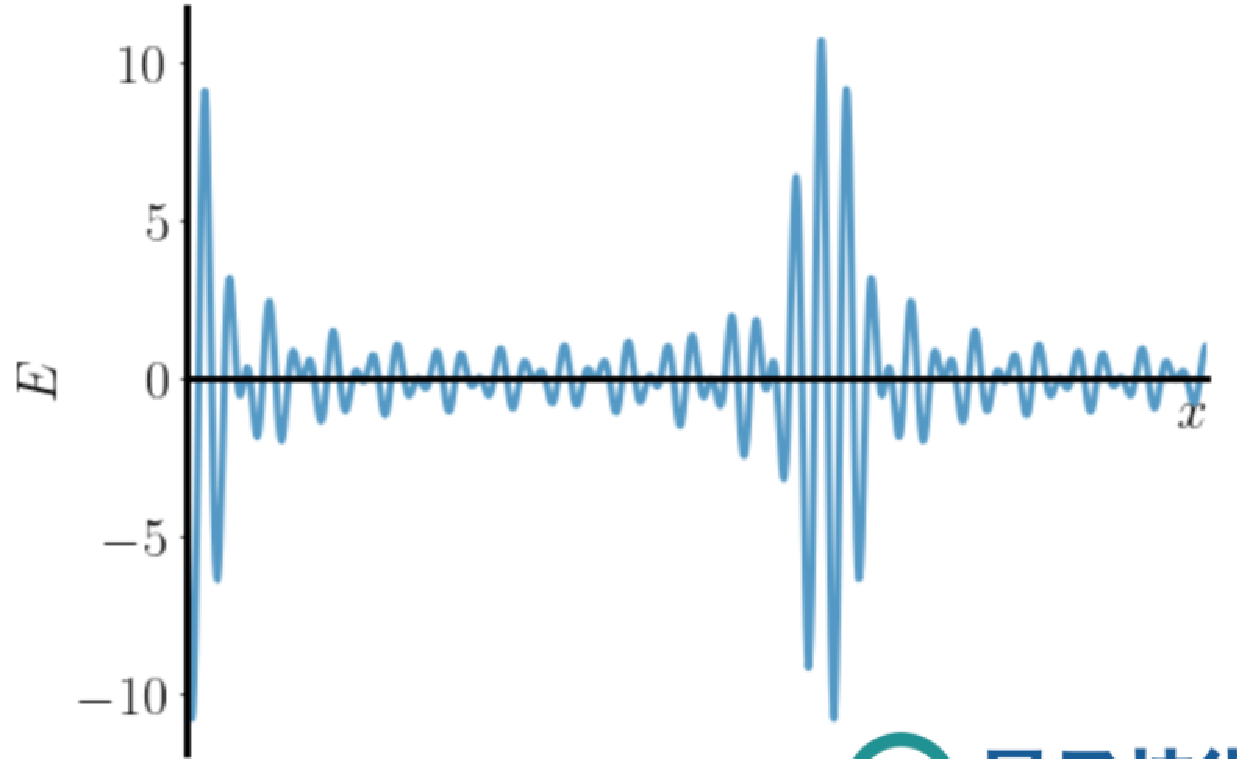
\includegraphics[width=0.8\textwidth]{lesson6/pulse.pdf}
    \label{fig: 1}
    \begin{center}
        \caption{複数の波の重ね合わせ状態}
    \end{center}
\end{figure}
これが簡単な例なんですけれども、真ん中のところには細かい振動があって、
突然大きな振幅が出てきて、その後また低いところに戻りますよね。これでいろんな形を作れるようになります。波はいくつかの足し算にすると\textbf{、振幅と周波数と位相が変わるようにできるなら、基本的にどんな関数でも作ることができます。}

そうすると、一番最初の例では、連続のsin波が続いていたんですけれども
それが永遠に続くなら、情報にはならないでしょ。情報として通信したい場合には、何か時間によって変調しなければなりませんね。こういう \textbf{pulse} になると情報として伝わるようになるかもしれません。そうすると、onとoff だけじゃなくて波の振幅と、ピークとピークの間の時間とか、いろんな手法があって、それを使って時間によって変動しないと message を伝えることはできません。



\section{単一光子との干渉}
\subsection{二重スリットの実験}

実験をちょっと見てみましょう:
% double_slit standard
\begin{figure}[H]
   \centering
    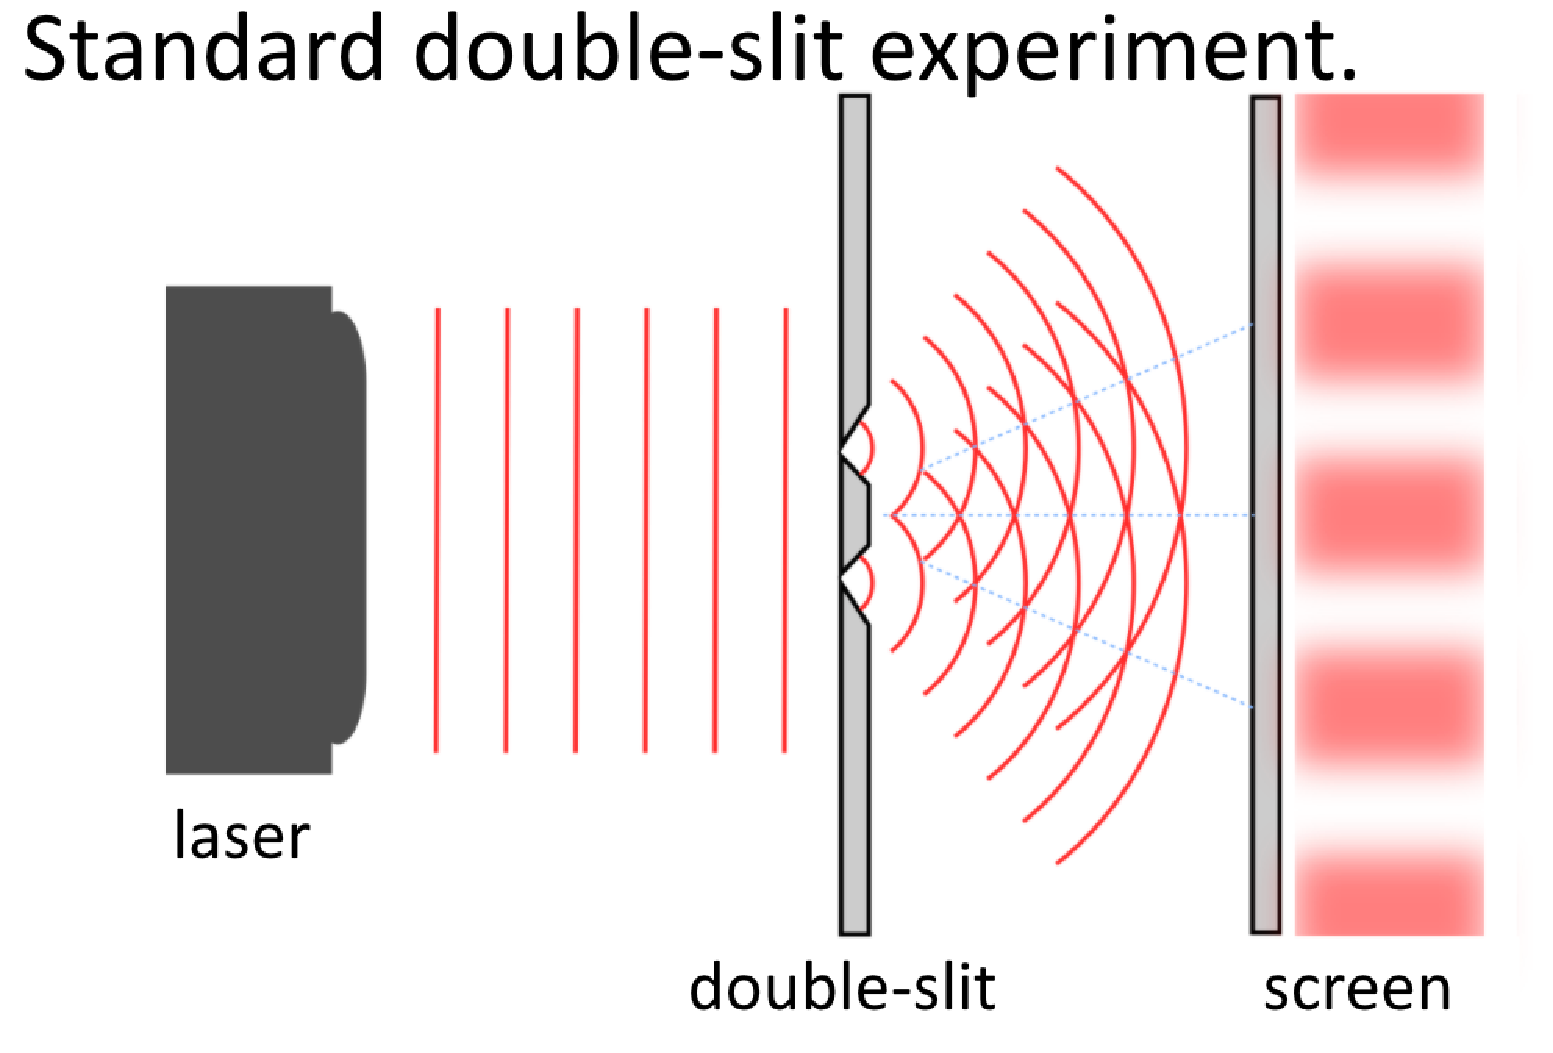
\includegraphics[width=0.8\textwidth]{lesson6/standard_double_slit.pdf}
    \label{fig: 1}
    \begin{center}
        \caption{二重スリットの実験}
    \end{center}
\end{figure}

これが\textbf{二重スリットの実験}なんですけれども左のはレーザーなので、そっちから出てくる光はコヒーレントな光というのが位相が見える状態になっているでしょう。例えば赤い線があるところには波の最大のところなので、プラスの方向でそれを考えてみましょう。光はレーザーから右に進んでくるんですが壁に当たって、この壁には二つの穴が空いています。この二つの穴を \textbf{double-slit} と言いますけ。でそこから波が出てきますが、形は変わるでしょう。これがカーブになるんでだんだん光は進んでいってスクリーンに当たります。このスクリーンは昔の実験では写真のフィルムを使っていたんですが現在では電子装置を使っているかもしれないですがそういうふうに見ていきましょう。

レーザーから光が出てくる右側にあるパターンが出てきます。明るいところと暗いところがある状態になるんですがこの場合には、バックグラウンドが白いので、白いところには光子が当たらないと考えてください。この赤いところとしては光が当たるところでそのスクリーンの色が変わるところです。

ではなぜ、こういうパターンになるんでしょう?これが干渉になるんです。こういう図で考えてみましょう:
% constructive interference
\begin{figure}[H]
   \centering
    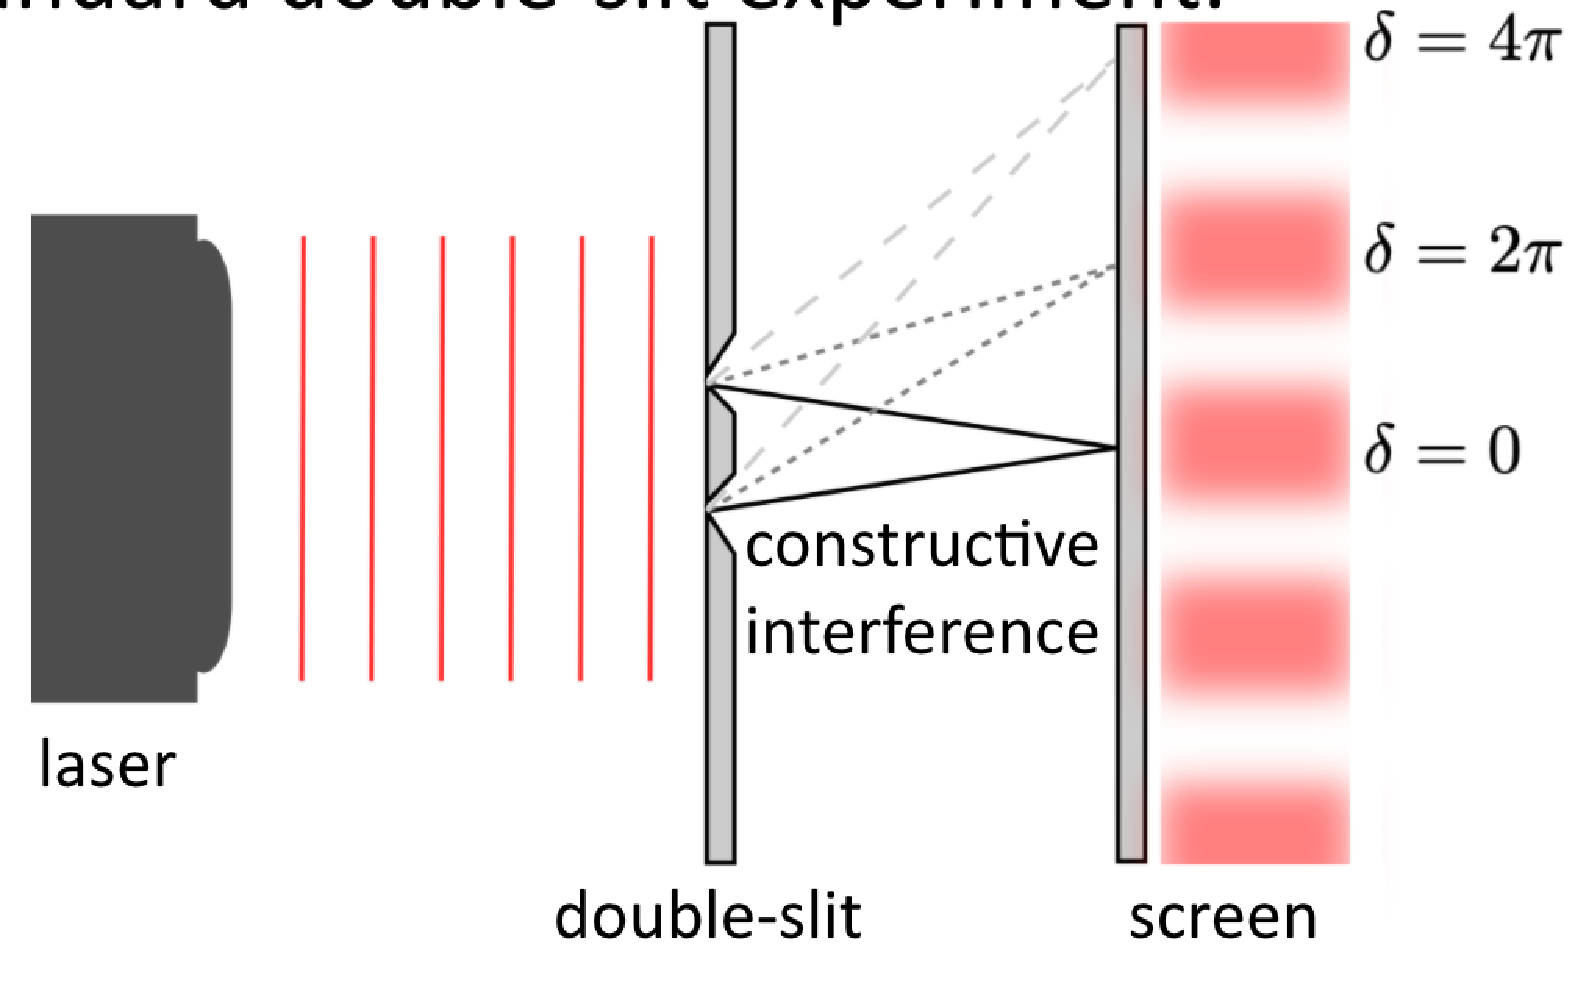
\includegraphics[width=0.8\textwidth]{lesson6/double_slit_constructive.pdf}
    \label{fig: 1}
    \begin{center}
        \caption{強め合い干渉}
    \end{center}
\end{figure}

これがその geometry としてはあるところには、上のslitと下のslitから出てくる光の距離は違ってきますね。で、真ん中のところだったら、slitまでの距離は一緒なのですが、
斜めに出てくると、その二つの経路の長さは違うんですね。じゃあ、そうすると、距離が一緒だったら、真ん中では、波の位相が合うようになりますから、位相がない場合は、波が足し算になりますね。\textbf{それが、普通には強め合い干渉になります}光は強くなるんでしょうでもそれが真ん中のところでは、$\delta = 0$ と書いてあるところなんですがそれだけじゃなくて、位相は$2\pi$違っていたら、それが一周回りますが、そうすると、位相が戻ってきて、また位相がまた一緒になりますね。\textbf{そうすると、
$\delta = 0$、$\delta = 2\pi$、$\delta = 4\pi$のところには、
各ところでは、干渉が強め合うことになります。}

逆の方向としては、その位相の差が$\pi$または$3\pi$になるところではそれが一つの波はポジティブと一つの波はネガティブになっているので、足し算にすると消えてしまいますよね:
% destructive inteference
\begin{figure}[H]
   \centering
    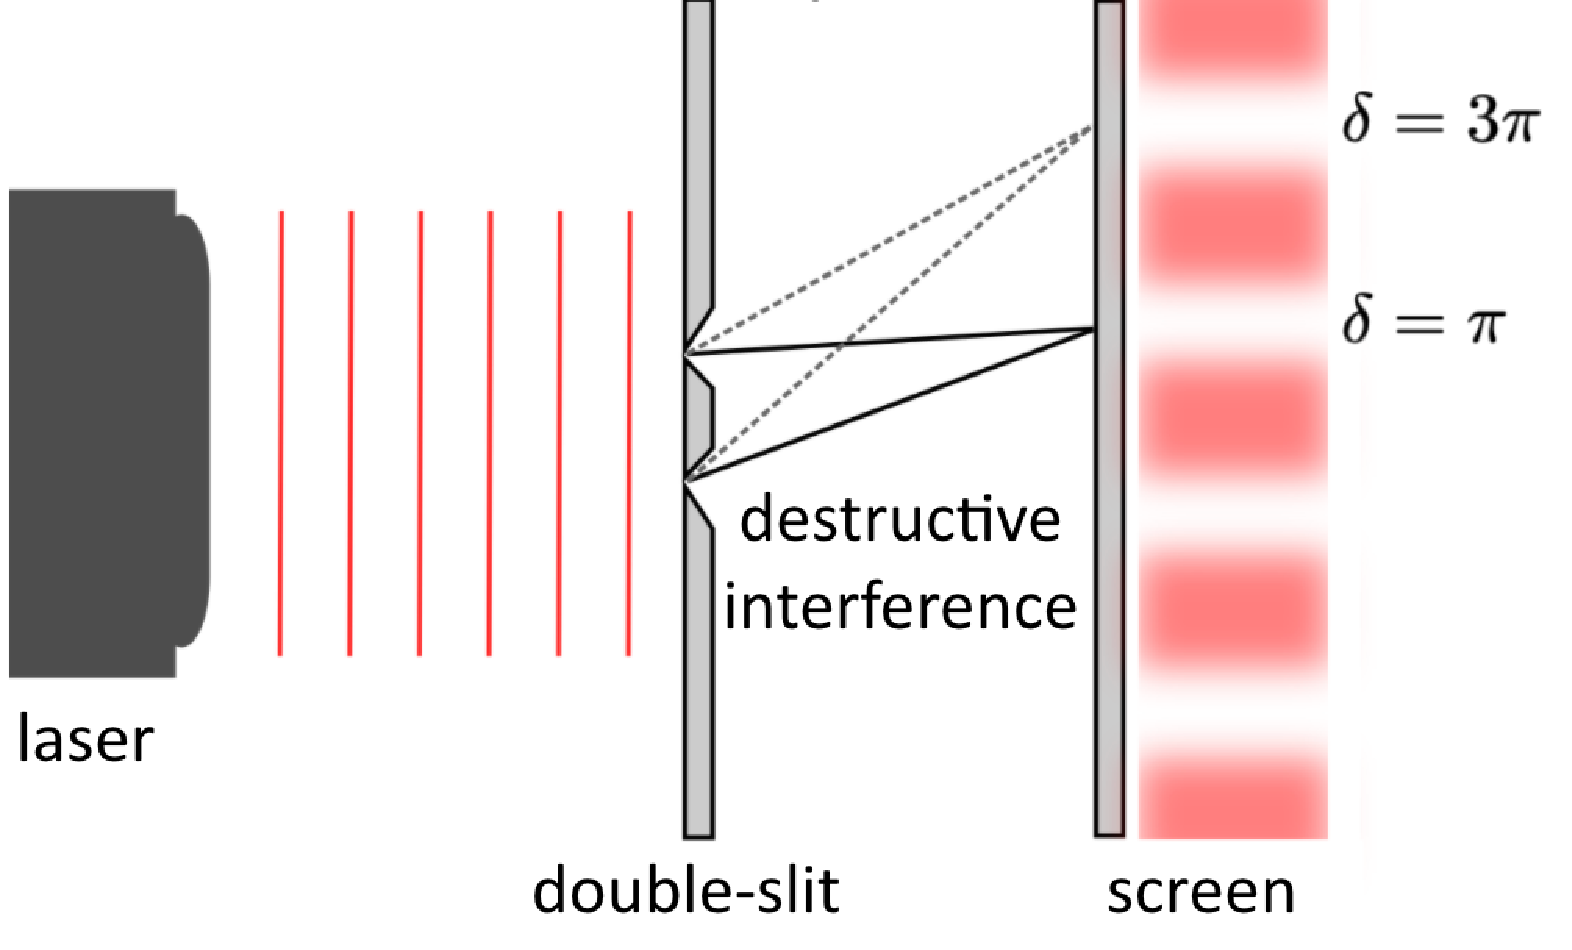
\includegraphics[width=0.8\textwidth]{lesson6/double_slit_destructive.pdf}
    \label{fig: 1}
    \begin{center}
        \caption{弱め合う干渉}
    \end{center}
\end{figure}
$+1-1=0$ なので、それは一緒のことなんですが。 そうすると、これは弱め合う干渉ですね、destructive interferenceです。これがまあ、強い光を使っている場合ですね。これは昔から知られているんです。



\subsection{単一光子との干渉}
一つの有名なことですが
量子としては、波の性格とParticle (粒子) の性格両方があるんですけれどもそうすると、光が強い場合じゃなくて、単一の光子になってくると、どうなるんでしょう?
% attenuated laser
\begin{figure}[H]
   \centering
    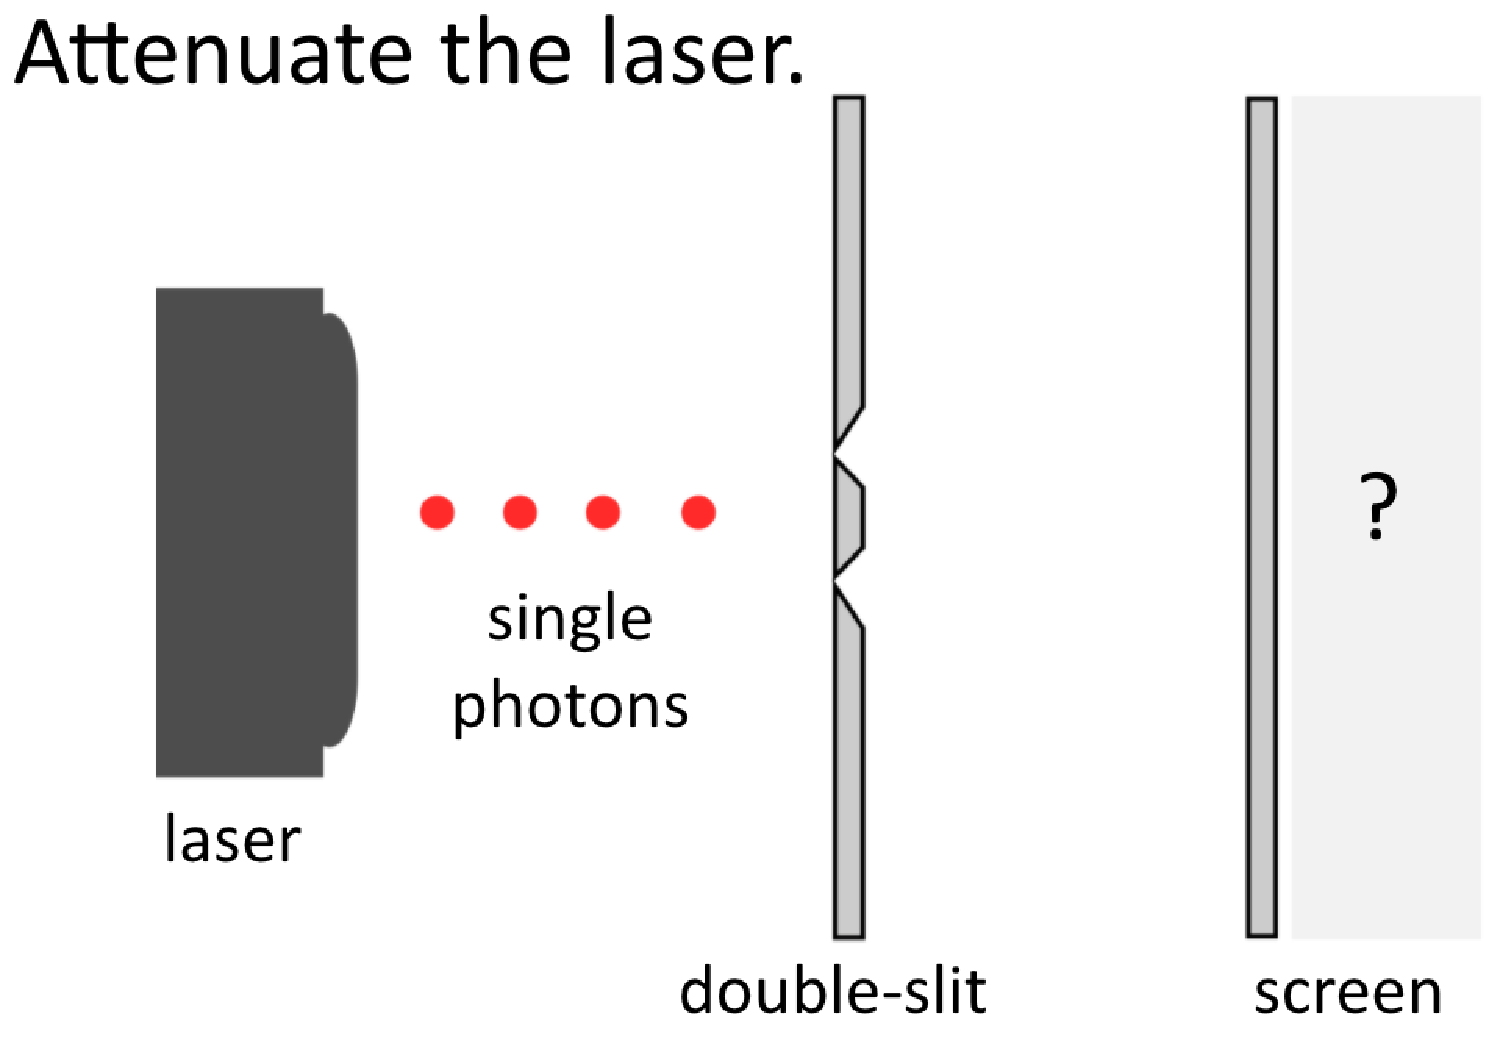
\includegraphics[width=0.8\textwidth]{lesson6/attenuate_laser.pdf}
    \label{fig: 1}
    \begin{center}
        \caption{減衰されたレーザの光}
    \end{center}
\end{figure}

まあ、最初にはそういうパターンはできるんですが、段々、レーザーが減衰した光になると、どうなるんでしょうかね?干渉としては、二つの波が必要なんだよね。でも、一つの光子は自分で二つの波になれるんでしょうかね?それとも、一つの波になるんでしょうかね?さて、どうなるんでしょう?
% block bottom
\begin{figure}[H]
   \centering
    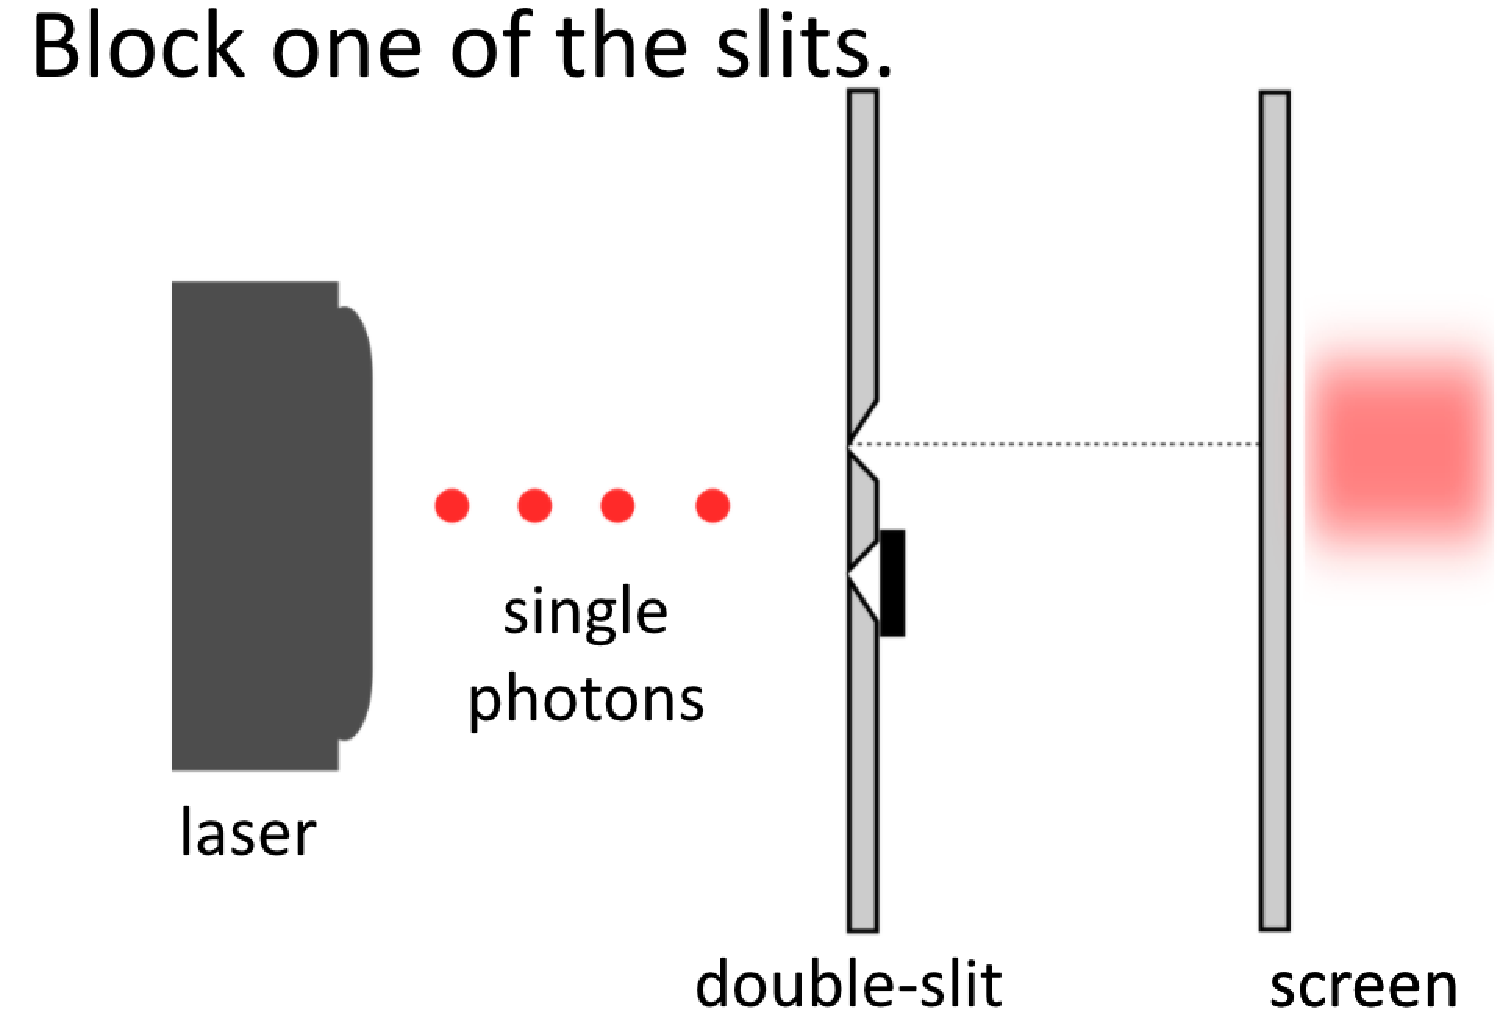
\includegraphics[width=0.8\textwidth]{lesson6/block_bottom.pdf}
    \label{fig: 1}
    \begin{center}
        \caption{下の穴を覆う}
    \end{center}
\end{figure}

例えば、一つだけのslitを通ると考えてみましょう。そうすると、こういうところでは、真っ直ぐにくる場合はあるかもしれないんですがちょっと曲がってしまうかもしれないんですが。まあこれが、標準分布の様子に見えますよね。
% block top
\begin{figure}[H]
   \centering
    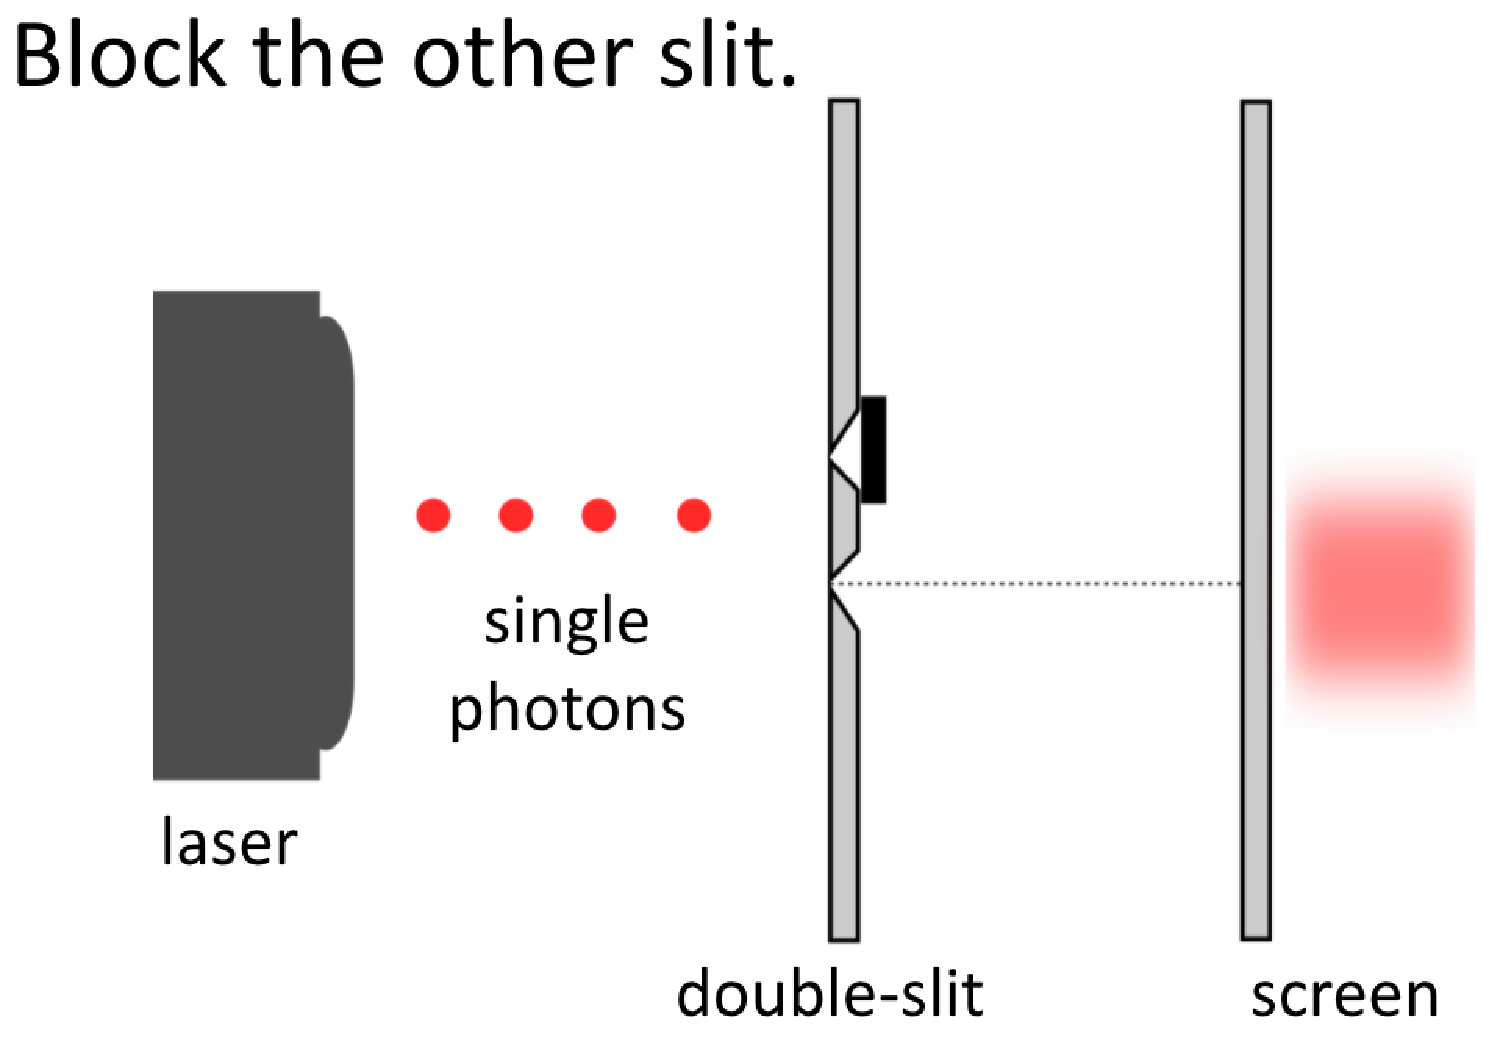
\includegraphics[width=0.8\textwidth]{lesson6/block_top.pdf}
    \label{fig: 1}
    \begin{center}
        \caption{上の穴を覆う}
    \end{center}
\end{figure}
さあ、上の図でご覧の通り、上のslitを通る場合には、例えば、
上のslitをしまうと、下のslitを通ってくると思いますので、合わせると、これも標準分布に見えますでしょう。真ん中のところが明るくて、上と下のところが暗いんだよね、光が当たらないで。

両方のslitを通るとどうなるのでしょう?
% block netiher expectation
\begin{figure}[H]
   \centering
    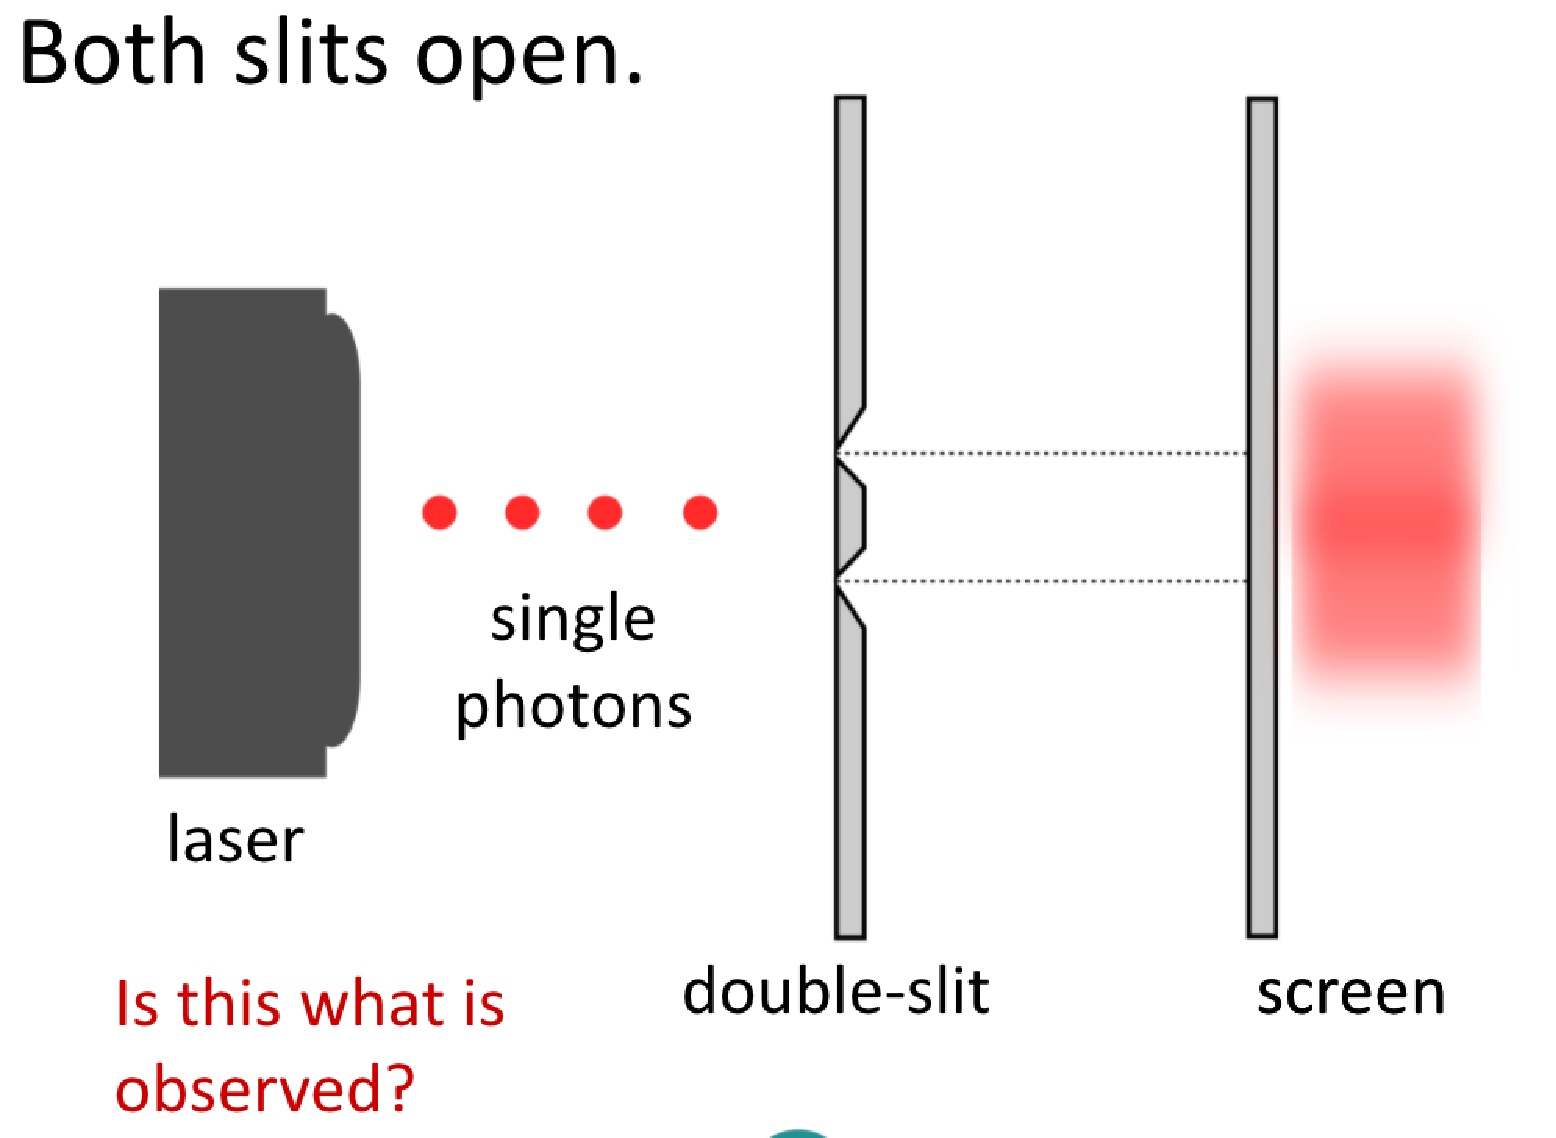
\includegraphics[width=0.8\textwidth]{lesson6/block_neither.pdf}
    \label{fig: 1}
    \begin{center}
        \caption{覆わない状態}
    \end{center}
\end{figure}
上の図は標準分布みたいなものの、足し算になると考えられると思いますけど、
これが、粒子一つなので、一つのslitだけを通ると考えたいんだよね。でも量子力学では効果が違うんだよね。そうすると、ちょっと見てみましょう。本当は、単一の光子は何百個あるので、一個ずつとってみましょうそうすると、スクリーンに当たるパターンは
こういうふうになります:
% block neither reality
\begin{figure}[H]
   \centering
    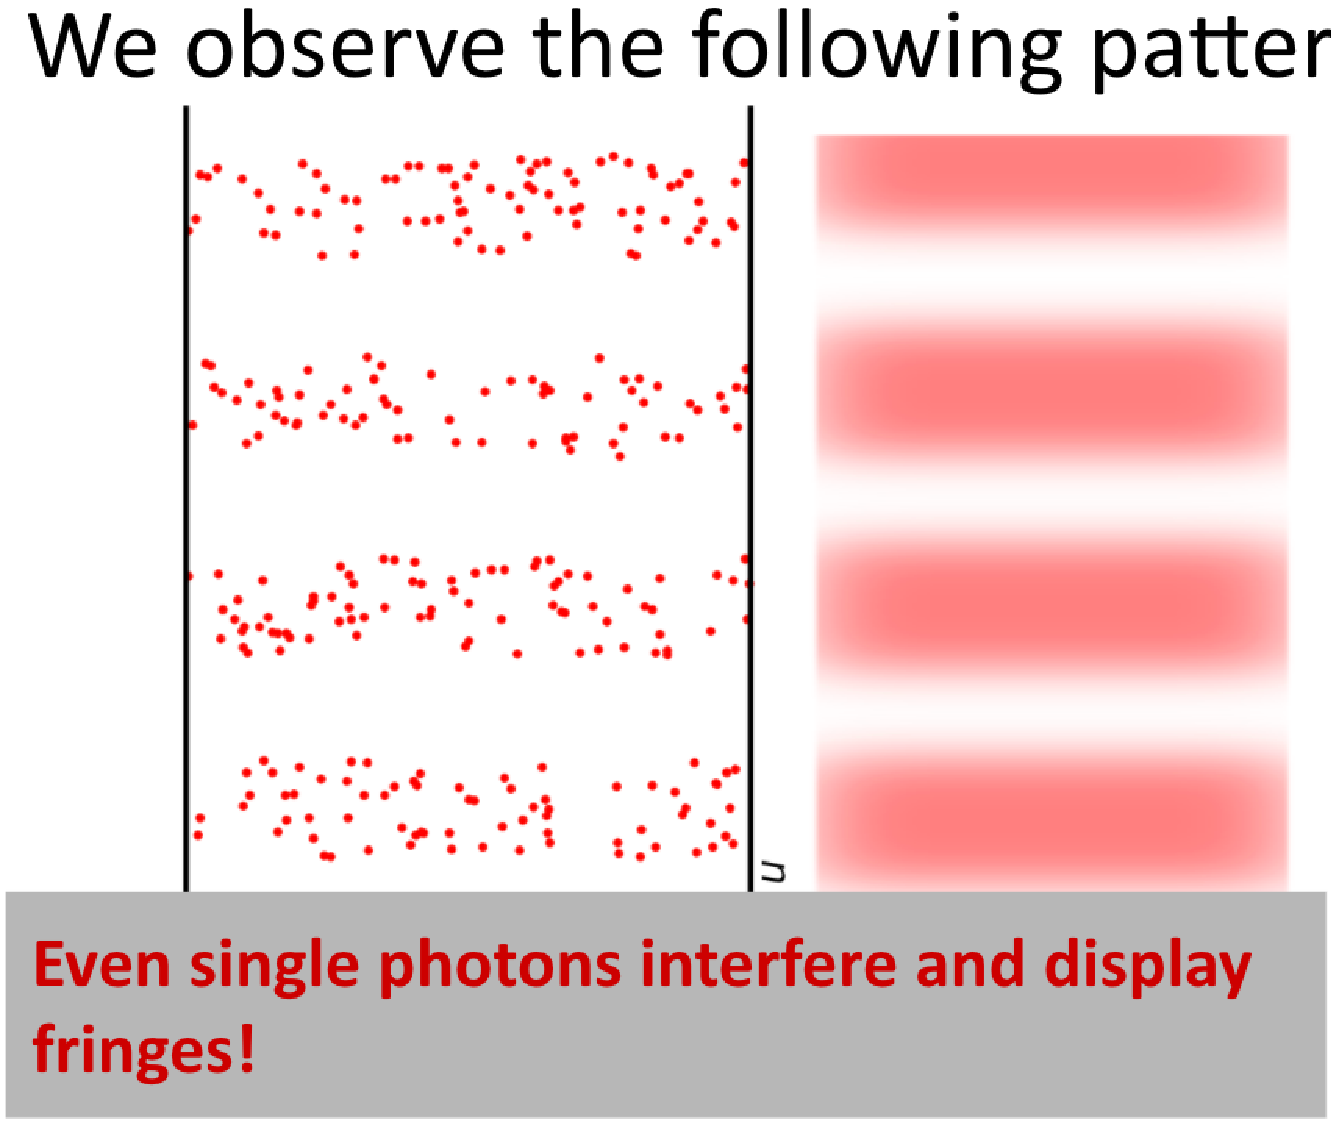
\includegraphics[width=0.8\textwidth]{lesson6/block_neither_reality.pdf}
    \label{fig: 1}
    \begin{center}
        \caption{覆わない状態:現実}
    \end{center}
\end{figure}
各ところには、あるところには光子が当たって次の光子は別のところに当たるんですけれど連続にすると、段々パターンが見えてきますよね。最初はランダムに見えるんですけれども時間が経つと、段々そのパターンがその模様が見えてくるんです。連続にすると、強い光と一緒になってこういう模様が出てきます。
パターンは、さっきのパターンと一緒なんですよね。\textbf{そうすると一つの光子は、自分としては干渉の状態になる可能性がありますというわけで、単一の光子も干渉は可能です。}



\section{量子ビットとの干渉}
この前のレッスンでは、アダマールゲートの効果を見ましたがそれについてもう一度考えてみましょう。例えばこういう場合だったら:
\begin{equation}
\begin{aligned}
|0\rangle &=\left(\begin{array}{l}
1 \\
0
\end{array}\right) \quad|1\rangle=\left(\begin{array}{l}
0 \\
1
\end{array}\right) \quad H=\frac{1}{\sqrt{2}}\left(\begin{array}{cc}
1 & 1 \\
1 & -1
\end{array}\right) \\
|0\rangle & \longrightarrow H|0\rangle=\frac{1}{\sqrt{2}}(|0\rangle+|1\rangle) \\
& \longrightarrow H\left[\frac{1}{\sqrt{2}}(|0\rangle+|1\rangle)\right] \\
&=\frac{1}{2}(|0\rangle+|1\rangle+|0\rangle-|1\rangle) \\
&=|0\rangle
\end{aligned}
\end{equation}

そうすると$\ket{0}$状態に一回アダマールをかけると、$\ket{+}$の状態が出てきます。$\ket{0} + \ket{1}$の状態が、normalization (規格化)の ために、割る $\sqrt{2}$になっています。もう一度アダマールをかけると、これが重ね合わせの状態でアダマールを$\ket{0}$の状態と$\ket{1}$の状態にかけてそうすると 、これが
$\frac{1}{2}(\ket{0}+\ket{1}+\ket{0}-\ket{1}$の二つの$\ket{0}$\textit{状態については(符号が)プラスなので一緒の位相なんですね}。そうすると 、それは強め合うことになります。
% 20:15 Aug 26

$\ket{1}$の状態については一つはプラスの位相になって
もう一つはマイナスの位相になっています。それは弱めあう、打ち消し合う干渉になります。そうすると 残りの状態は$\ket{0}$状態になりますね。これを\textbf{「干渉」}といいます。別の例として、インプットが$\ket{0}$状態ではなく$\ket{1}$状態の場合にはアウトプットの状態は $\ket{0}-\ket{1}$。つまり$\ket{1}$状態には$\pi$の位相、マイナスの位相になっています。もう一度アダマールをかけると足し算すると結果は$\ket{1}$状態になりますよね。これも干渉になります。2回アダマールをかけると初期状態に戻ります。
$$H H = I$$(アイデンティティの行列になります。
違う例をみてみましょう:
\begin{equation}
B S 1=\frac{1}{\sqrt{2}}\left(\begin{array}{cc}
1 & 1 \\
1 & -1
\end{array}\right) \quad B S 2=\frac{1}{\sqrt{2}}\left(\begin{array}{cc}
-1 & 1 \\
1 & 1
\end{array}\right) \quad B S 2 \cdot B S 1 \neq I
\end{equation}
二つのゲートを使います一つは$BS1$、もう一つを$BS2$と呼びましょう。
二つともユニタリ演算なんですが$BS2 BS1 = I $(アイデンティティ) ではありません。ではどうなるでしょうか:
\begin{equation}
\begin{aligned}
B S 2 \cdot B S 1|1\rangle &=B S 2 \cdot \frac{1}{\sqrt{2}}\left(\begin{array}{cc}
1 & 1 \\
1 & -1
\end{array}\right)\left(\begin{array}{l}
0 \\
1
\end{array}\right) \\
&=B S 2 \cdot \frac{1}{\sqrt{2}}\left(\begin{array}{c}
1 \\
-1
\end{array}\right) \\
&=\frac{1}{2}\left(\begin{array}{cc}
-1 & 1 \\
1 & 1
\end{array}\right)\left(\begin{array}{c}
1 \\
-1
\end{array}\right) \\
&=\frac{1}{2}\left(\begin{array}{c}
-2 \\
0
\end{array}\right)=-|0\rangle=|0\rangle
\end{aligned}
\end{equation}

出てくる結果がグローバルな位相は最終的な結果に影響を与えないので$\ket{0}$状態になります。$BS1$をかけて、$BS2$をかけて$\ket{1}$状態に作用させると結果は$\ket{0}$状態になります。つまり、この二つを合わせるとNOTゲートと同じになります。
\subsection{Mach-Zehnderの干渉器}
光子を例にとって見てみましょう:
% Mach-Zehnder set-up
\begin{figure}[H]
   \centering
    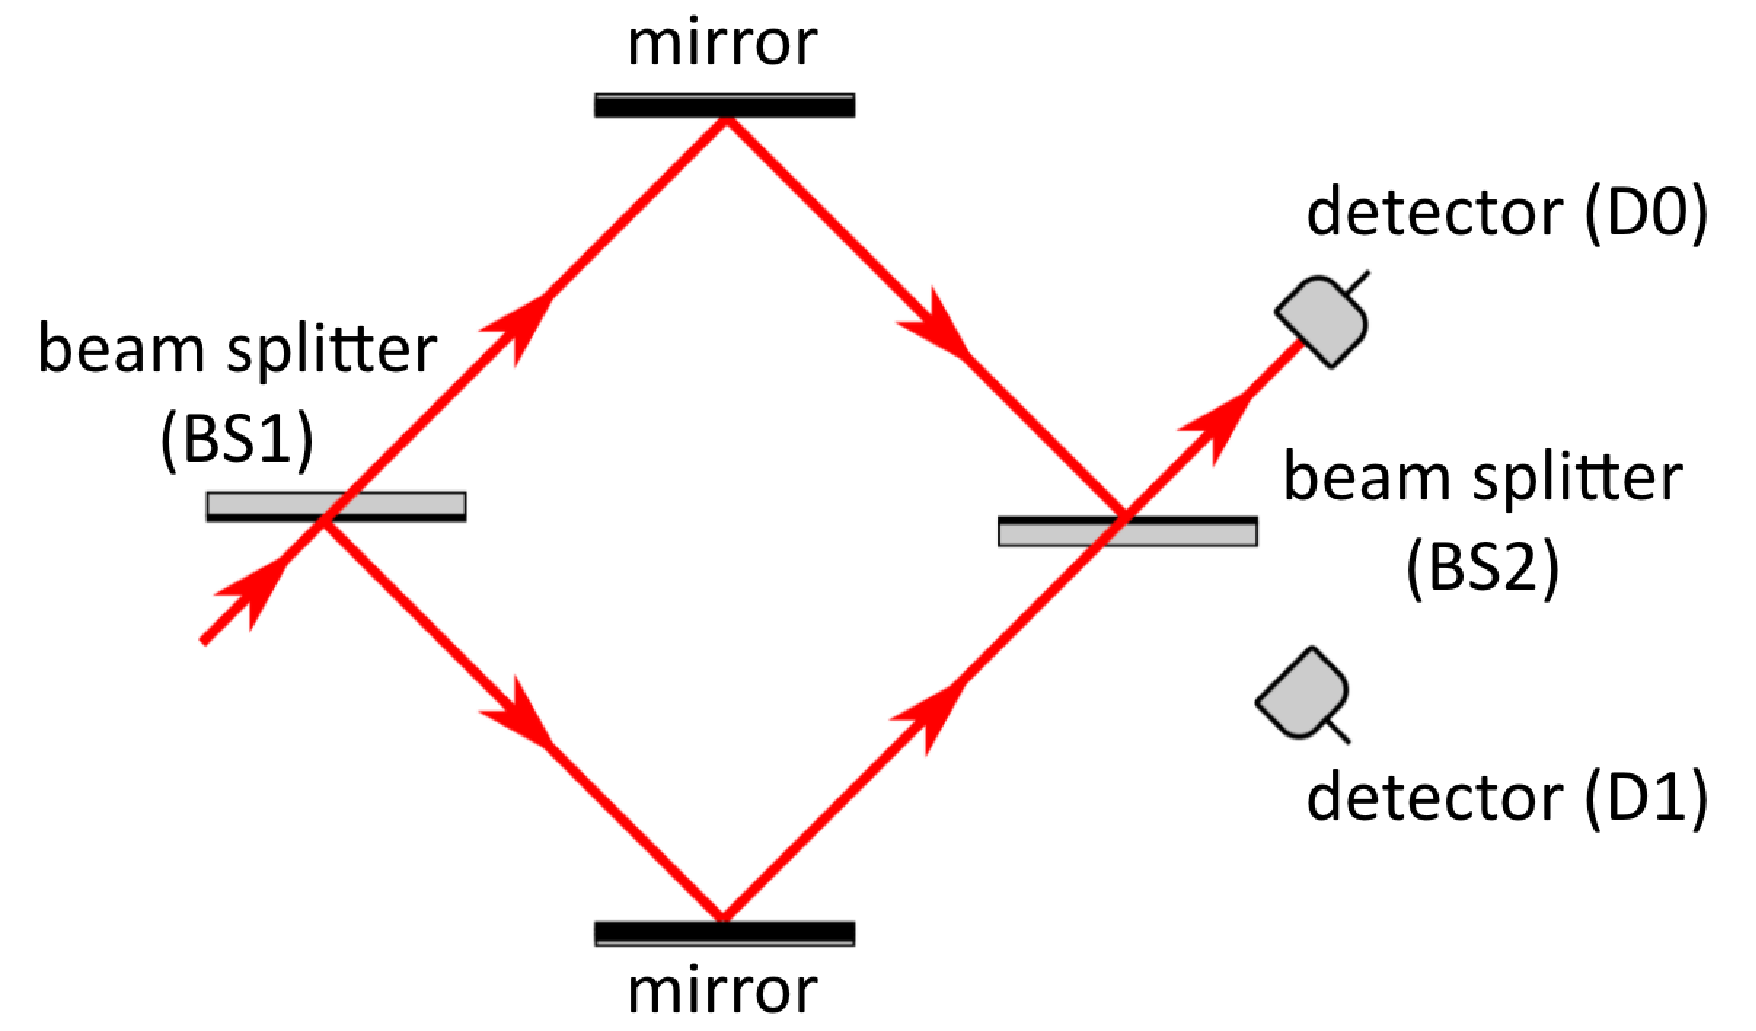
\includegraphics[width=0.8\textwidth]{lesson6/mach_zehnder.pdf}
    \label{fig: 1}
    \begin{center}
        \caption{Mach-Zehnderの干渉器}
    \end{center}
\end{figure}

有名な実験として\textbf{Mach-Zehnderの干渉器}が知られています。二つの鏡と二つのビームスプリッターと二つのディテクター(検知器)。さっきのBS1、BS2はビームスプリッターに対応しています。今回は数学としては完全ではなく
簡単に表現していますが印象になると思います。この六つの装置に、光子を入れます。強いレーザーのような光を入れると半分の光は上に行って。もう半分は下に行きます。上の光は鏡に当たって、またビームスプリッターに当たって下の光も鏡に反射して、ビームスプリッターを通って。でもこの図を見ると二つのディテクター(検知器)があるでしょう。これがディテクター0(D0)とディテクター1(D1)。\textit{出てくる光はディテクター0にしか当たりません}。なぜかというと、二つ目のビームスプリッターで干渉します。上に行く光が強め合う干渉、下に行く光が弱め合う干渉になって上のディテクター(検知器)だけに光が当たります。

単一の光子の場合はどうなるでしょうか。概念としてはさっきのステップと同じですが単一の光子が干渉の概念も含む場合があります。ちょっとみてみましょう:
% Single photon Mach-Zehnder case
\begin{figure}[H]
   \centering
    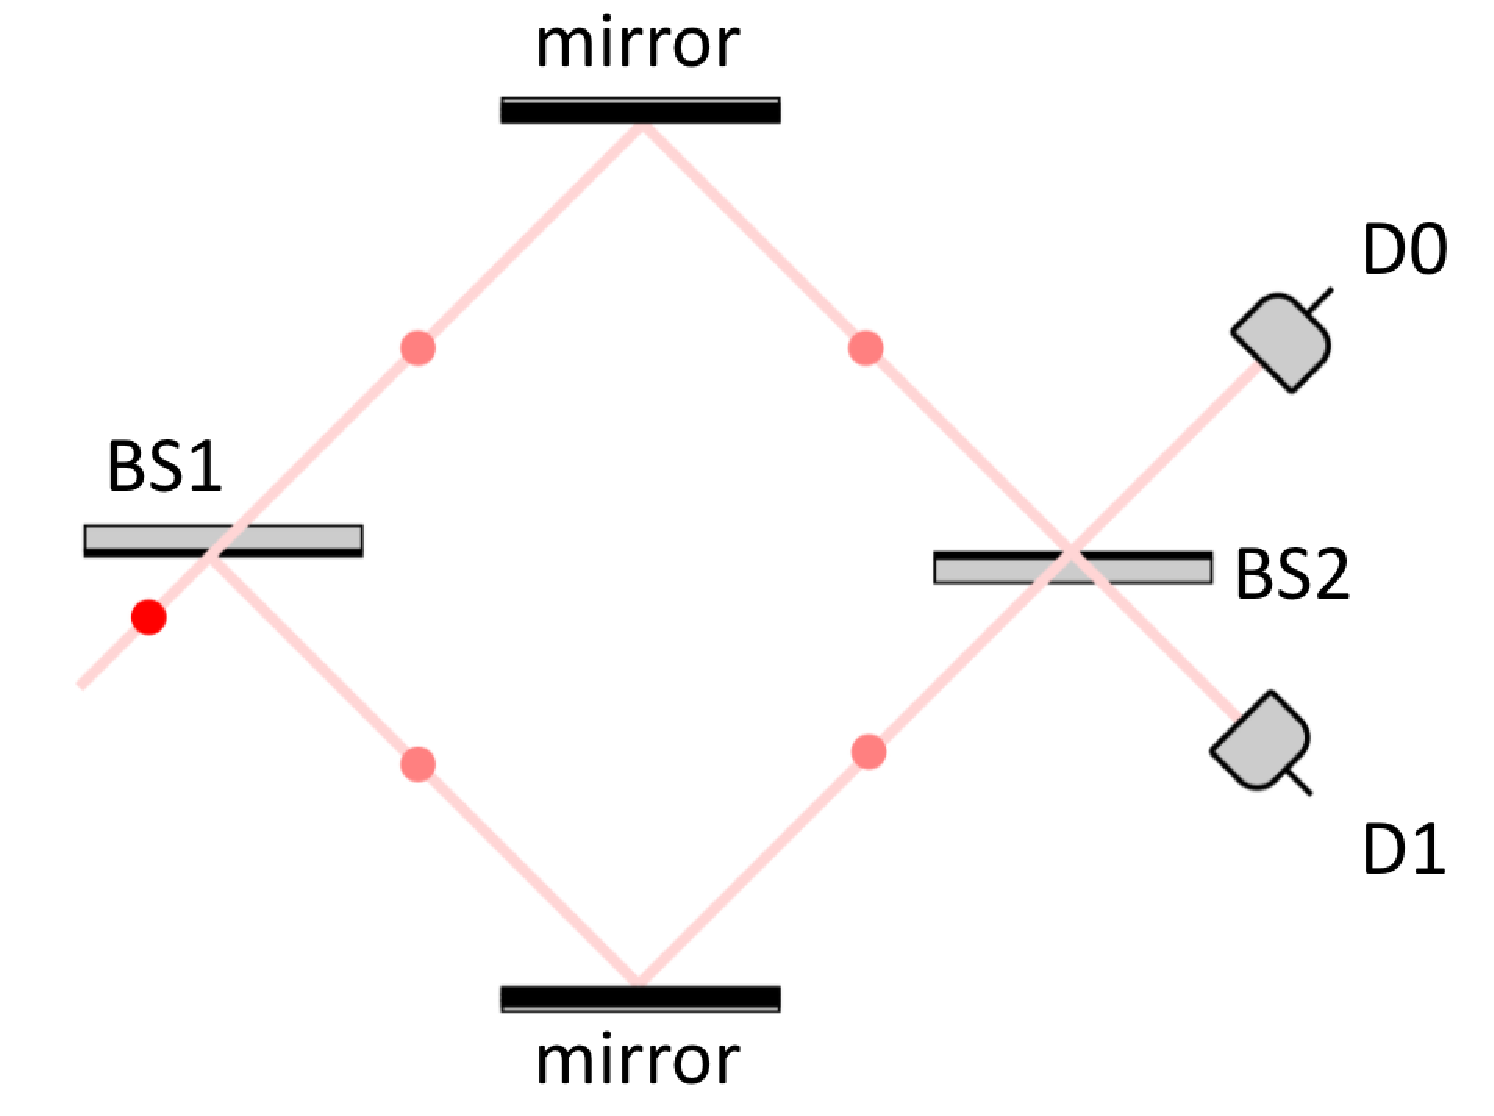
\includegraphics[width=0.8\textwidth]{lesson6/mach_zehnder_single_photon.pdf}
    \label{fig: 1}
    \begin{center}
        \caption{Mach-Zehnderの干渉器:単一光子}
    \end{center}
\end{figure}

この場合にはどちらのディテクターにクリックするでしょうか?上の$D0$でしょうか、それとも下の$D1$でしょうか?
この場合、Qubitの定義として$\ket{0}$の基底状態と$\ket{1}$の基底状態はどのように定義すればいいでしょうか?簡単な例としては上に光子がある場合、これを$\ket{0}$状態と呼びましょう:
% 0 ket top
\begin{figure}[H]
   \centering
    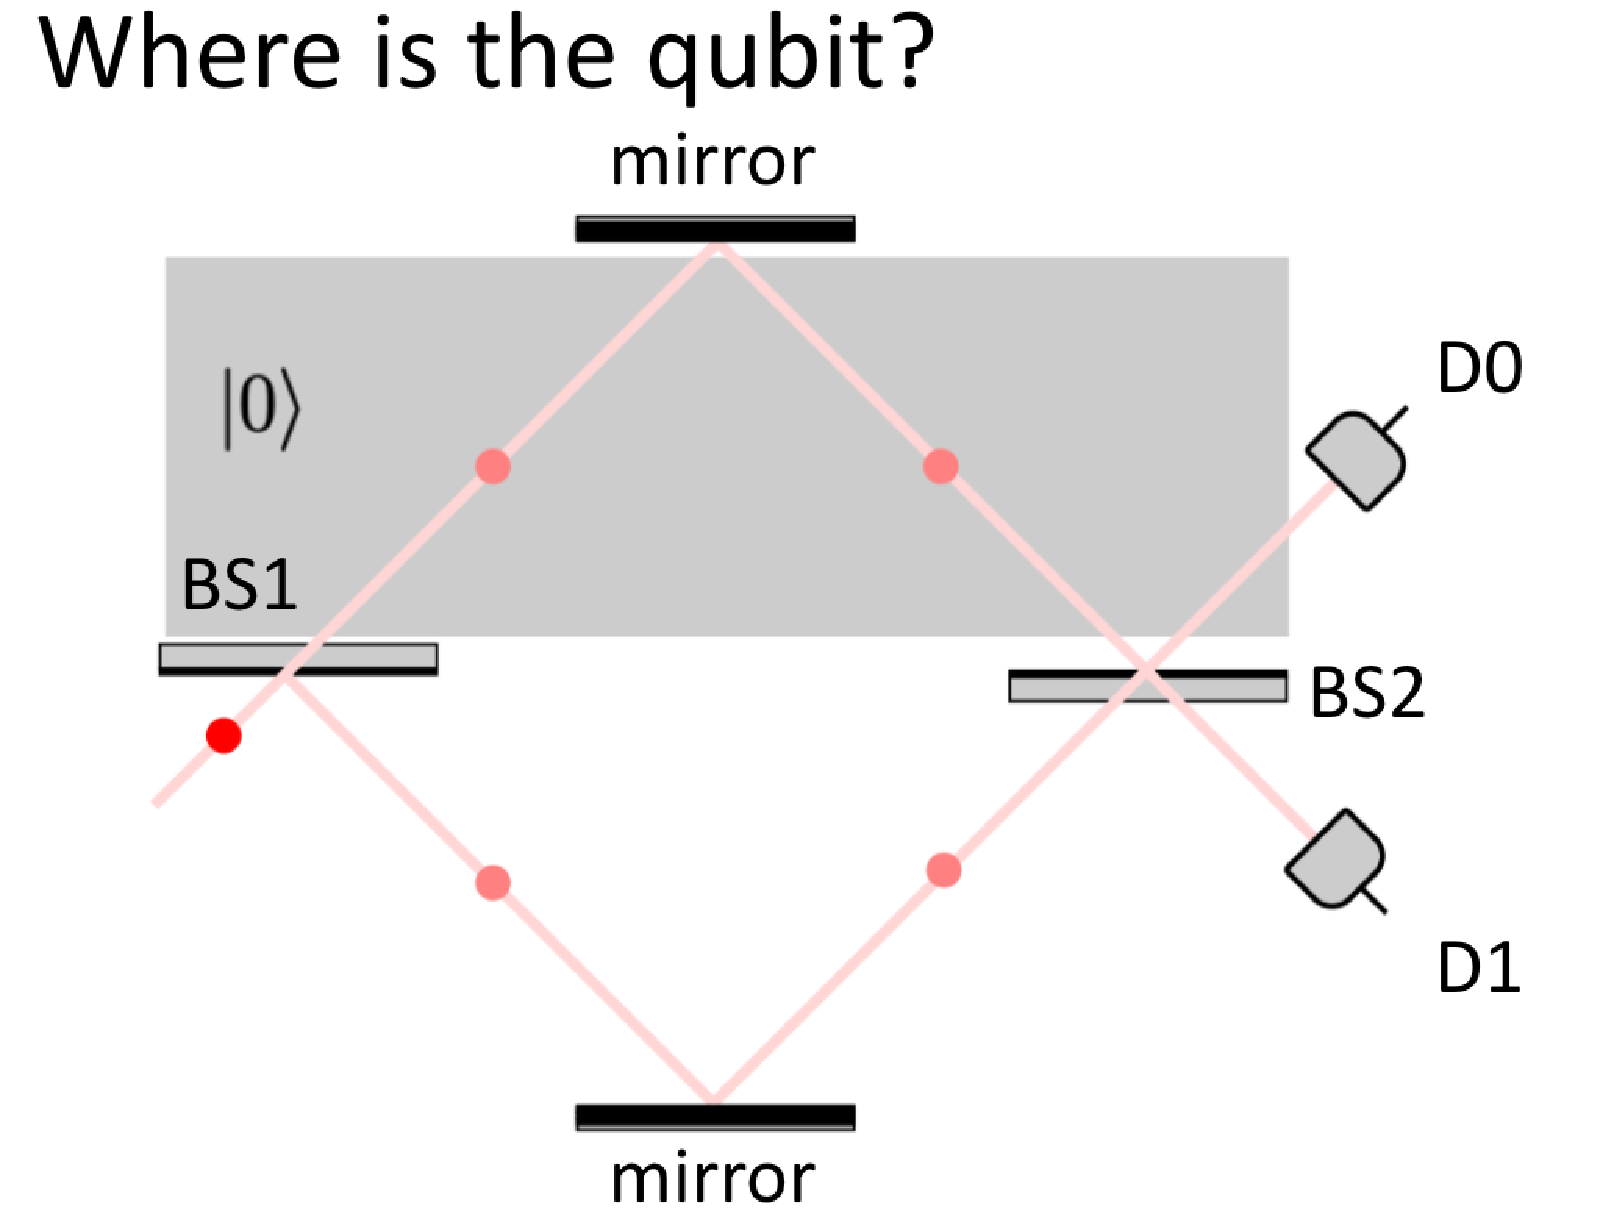
\includegraphics[width=0.8\textwidth]{lesson6/0_ket_botttom.pdf}
    \label{fig: 1}
    \begin{center}
        \caption{$\ket{0}$の状態}
    \end{center}
\end{figure}

下の経路にある場合はこれを$\ket{1}$状態と呼びましょう:
% 1 ket bottom
\begin{figure}[H]
   \centering
    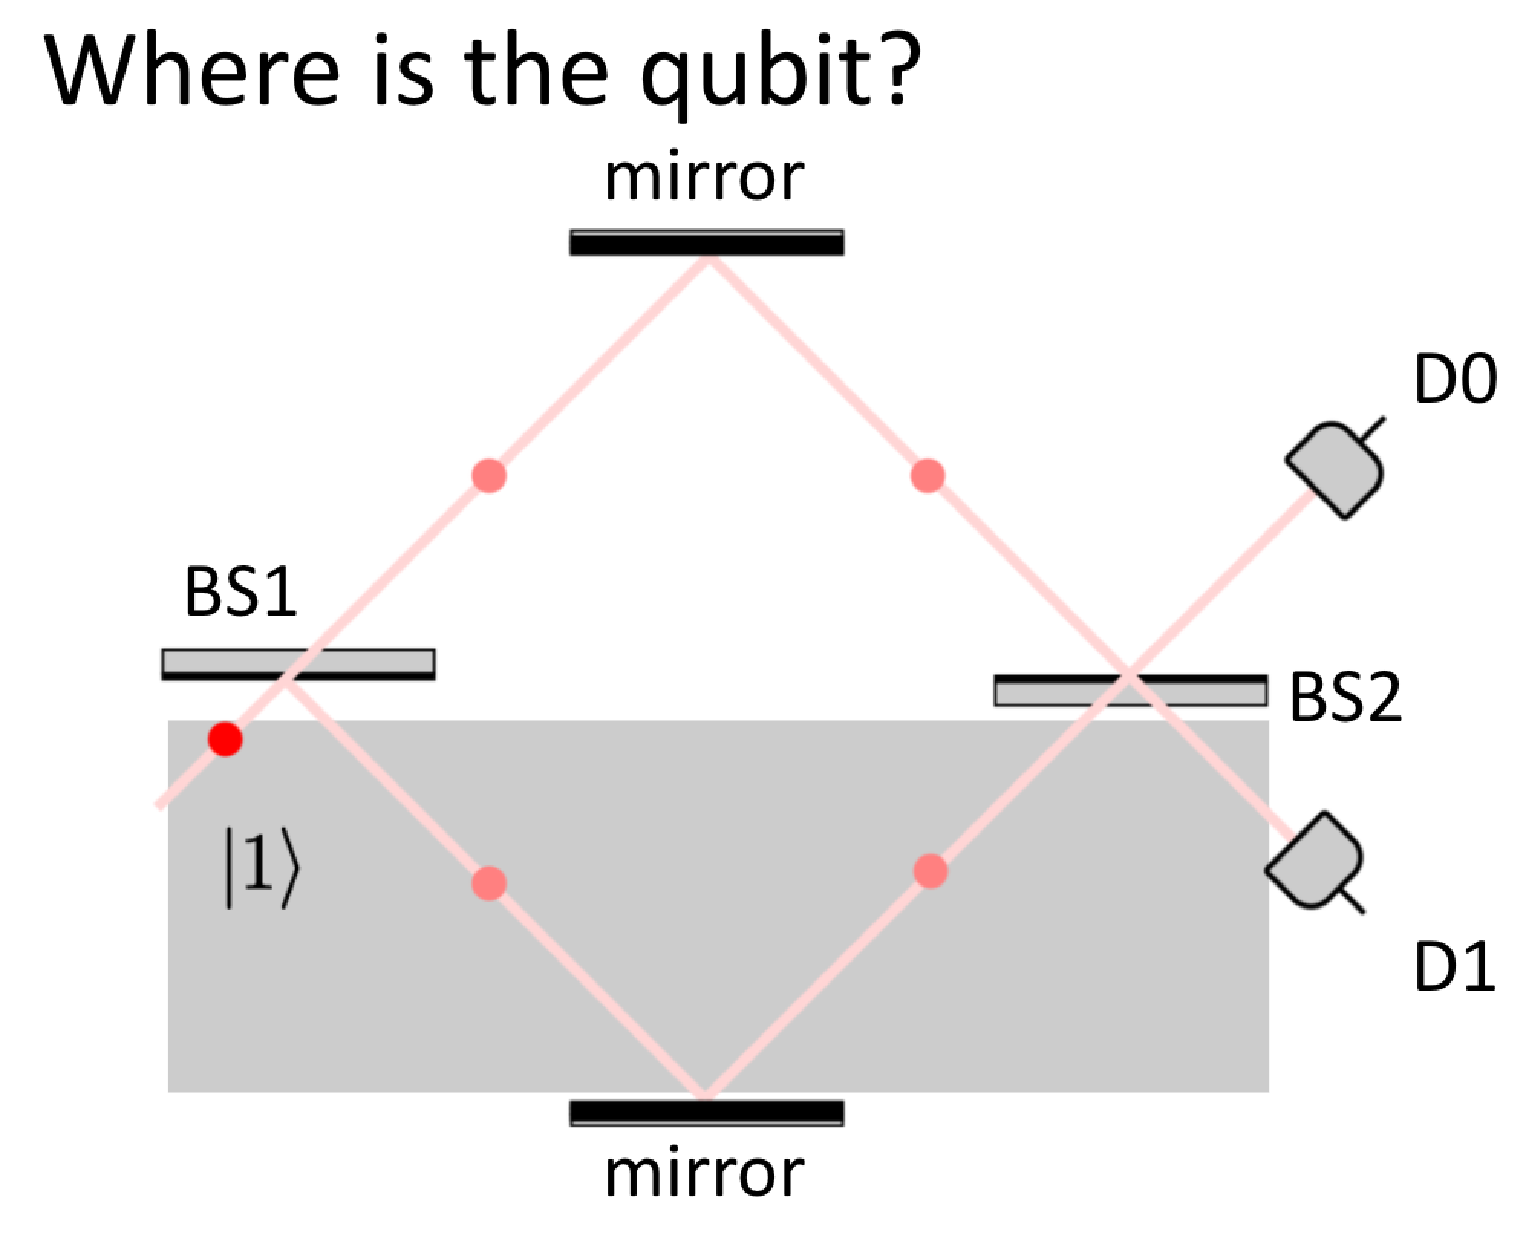
\includegraphics[width=0.8\textwidth]{lesson6/1_ket_bottom.pdf}
    \label{fig: 1}
    \begin{center}
        \caption{$\ket{1}$の状態}
    \end{center}
\end{figure}

最初のインプットの光子が下の経路にありますのでこれを$\ket{1}$の状態と呼んでこういう数式があったでしょ:
\begin{equation}
B S 2 \cdot B S 1|1\rangle=|0\rangle
\end{equation}
この数式で$BS1$と$BS2$の効果を光子の状態としての計算することができます。

\textbf{この場合、必ずD0がクリックします}:
% D0 always clicks
\begin{figure}[H]
   \centering
    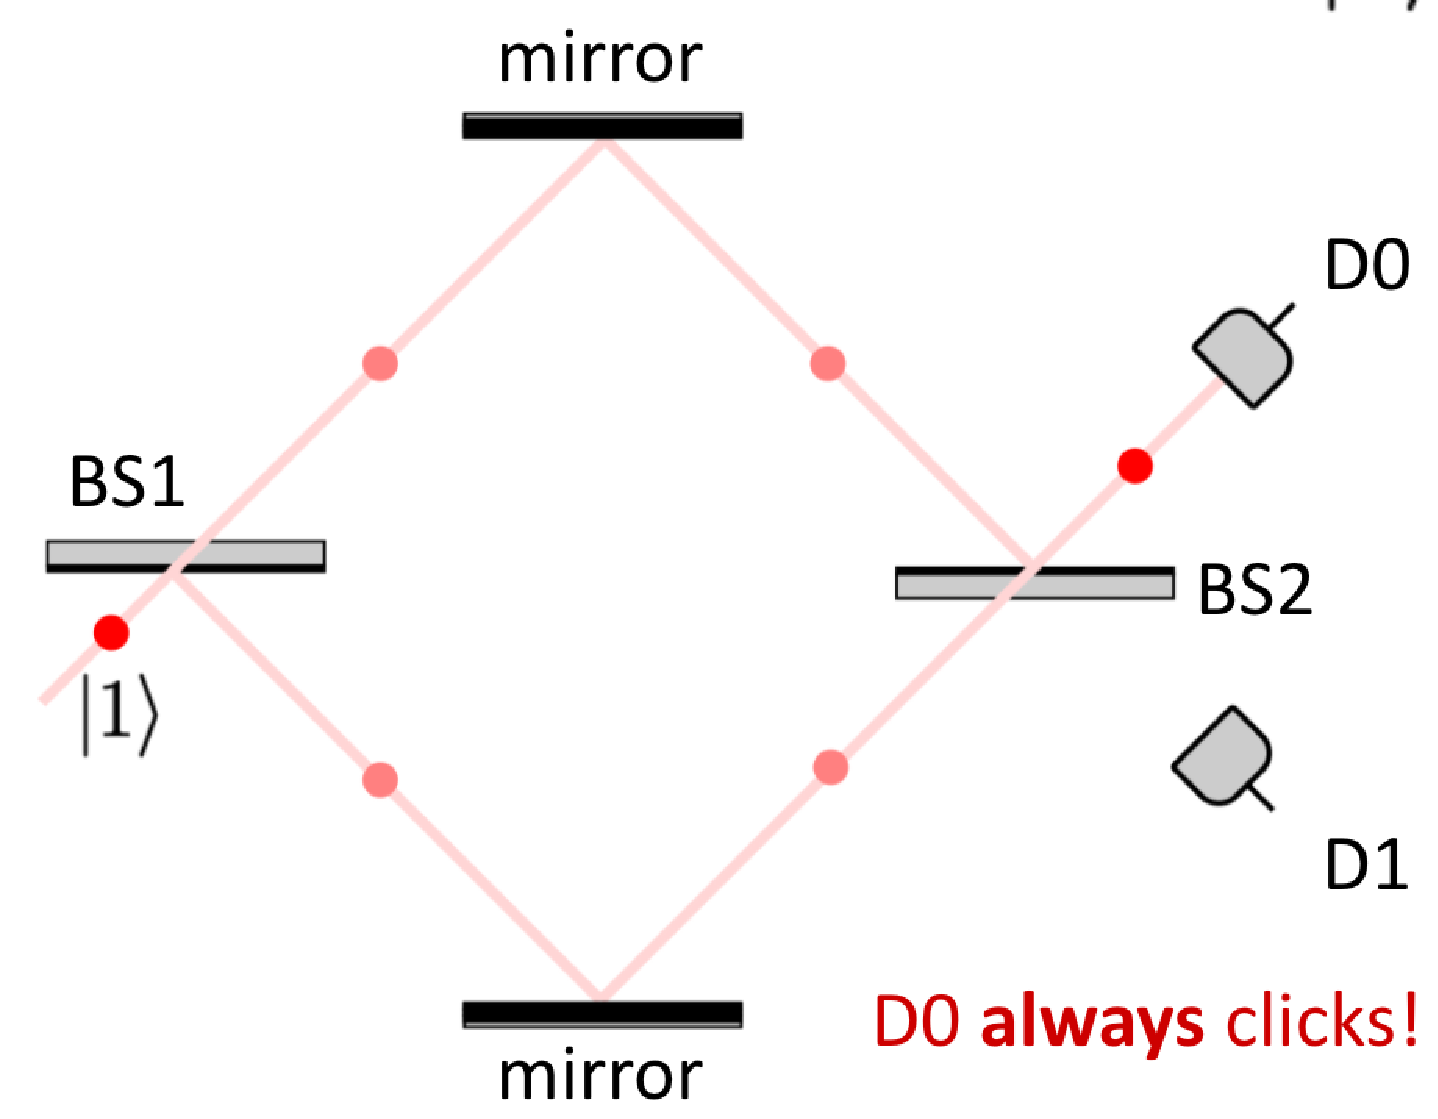
\includegraphics[width=0.8\textwidth]{lesson6/d0_always_clicks.pdf}
    \label{fig: 1}
    \begin{center}
        \caption{$D0$100\%確率}
    \end{center}
\end{figure}

$D1$にクリックする確率は0\%で$D0$にクリックする確率は100\%になります。この前の例(ヤングの実験)では二重スリットに当たって複雑な模様になっていましたが。

ではちょっとだけ条件を変えましょう:
% block bottom path
\begin{figure}[H]
   \centering
    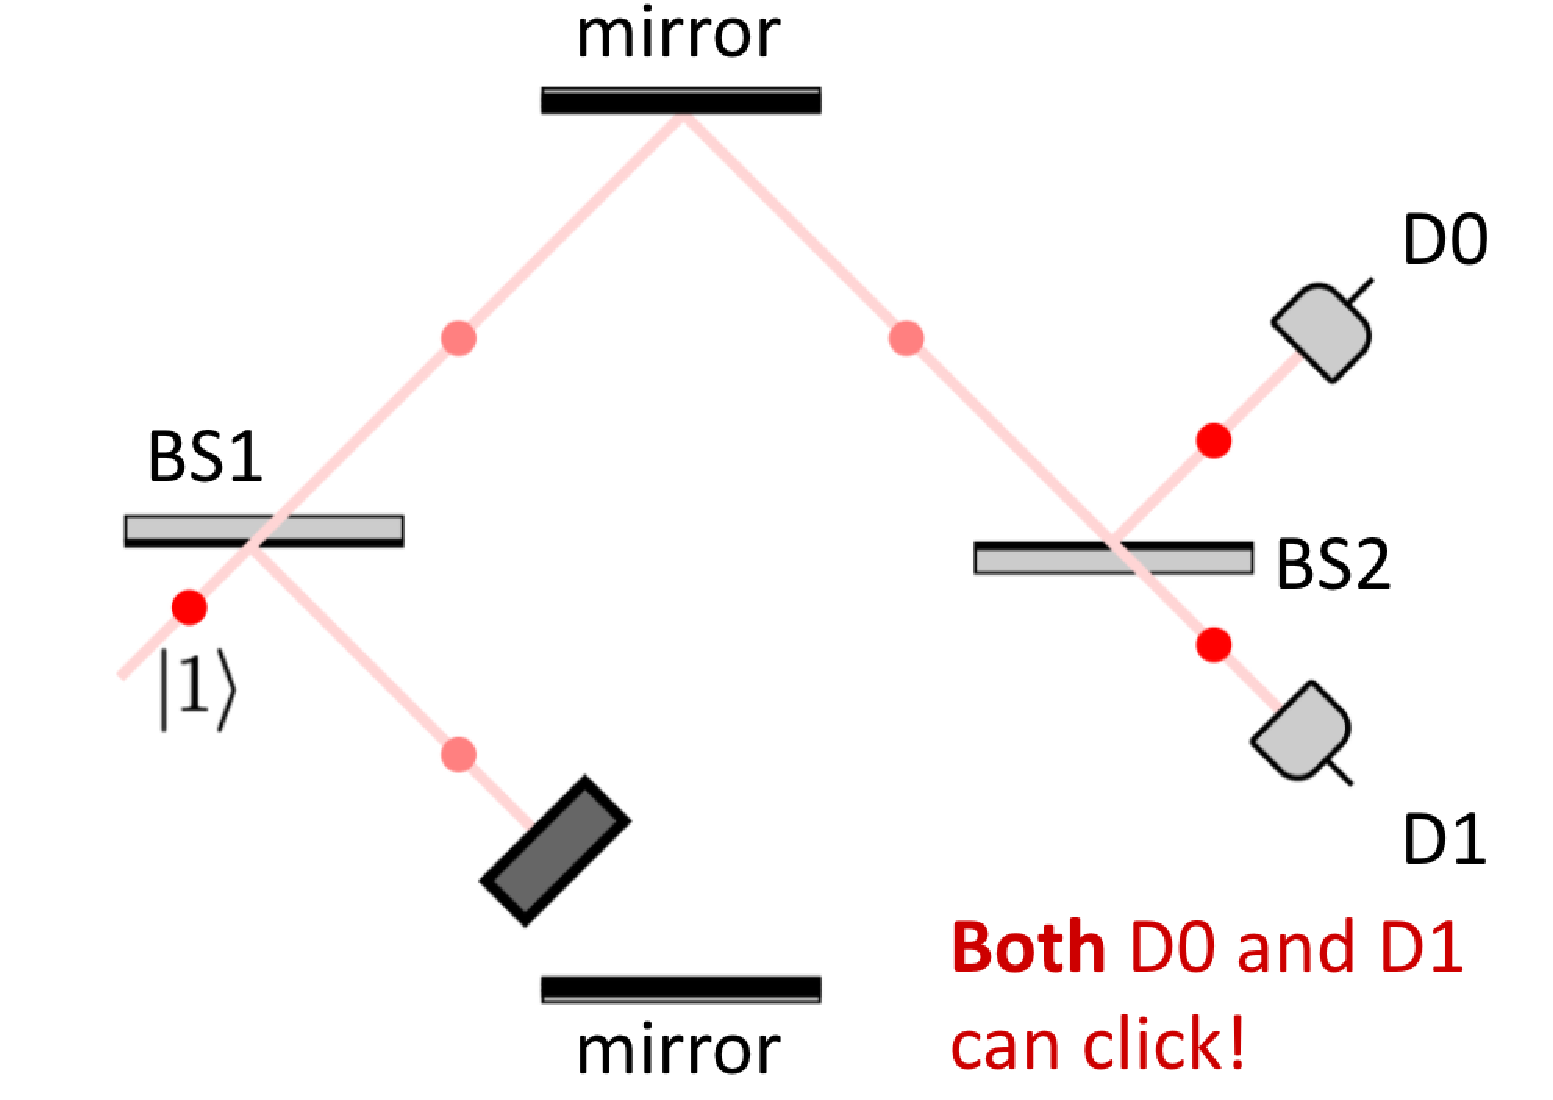
\includegraphics[width=0.8\textwidth]{lesson6/bottom_blocked.pdf}
    \label{fig: 1}
    \begin{center}
        \caption{下の経路を塞ぐ}
    \end{center}
\end{figure}
さっきの例では下の経路では鏡に当たってこの部分($BS2$)で干渉していたんですけれどもこの例では、経路の途中に何か物を置いて光子が通れないようにすると下に出てくる光子は最後のディテクターまで来れなくなります。そうすると どうなるでしょう?

上の経路しか残らないので(BS2の部分で)まだ分かれる可能性があって
上に行くか下に行くか、50:50 の状態になります。\textbf{半分の確率で$D0$と$D1$にクリックします。}

ですが、下に行くのは、最初のビームスプリッターに当たると下に行く確率振幅は、半分は下の経路と、半分は上の経路になるとその下のところに行くとそれはまた消してしまって、それが最後まで来る確率は半分にしかならない。

さっきの例で、必ず$D0$はクリックしていたんですが、それは100\%の確率で理想としてなんですがこの場合だったら、どっちかに来るという確率は50\%なので何も当たらない確率も50\%当たる確率の50\%の中には、半分は$D0$と半分は$D1$に当たります。

